\documentclass[a4paper,10pt]{article}
\usepackage{latexsym}
\usepackage{amsmath}
\usepackage{amssymb}
\usepackage{bm}
\usepackage{wrapfig}
\usepackage{fancybox}
\pagestyle{plain}

\begin{document}

Learning to Promote Saliency Detectors

Yu Zeng1 , Huchuan $\mathrm{L}\mathrm{u}^{1}$, Lihe Zh an $\mathrm{g}^{1}$, Mengyang Feng1, Ali Borji2 1 Dalian Unive rsi ty of Tec hnology, China

2 University of Central Florida, USA

zengyu@mail. dlut. edu. cn, lhchuan@dlut. edu. cn, zhanglihe@dlut. edu. cn,

mengyangfeng@gmail. com, aliborji@gmail. com

Abstract

{\it The categories and appearance of salient objects vary from image to image, therefore, saliency detection is an image-specific task. Due to lack of large-scale saliency training data, using deep neural networks} ({\it DNNs}) {\it with pre}- {\it training is difficult to precisely capture the image-specific saliency cues. To solve this issue}, $we$ formulate {\it a zero-shot learning problem to promote existing saliency detectors. Concretely, a DNN is trained as an embedding function to map pixels and the attributes of the salient}/{\it background regions of an image into the same metric space, in which an image-specific classifier is learned to} classify {\it the pix}- {\it els. Since the image-specific task is performed by the clas}- {\it sifier, the DNN embedding} effectively {\it plays the role of a general feature extractor. Compared with transferring the learning to a new recognition task using limited data, this formulation makes the DNN learn more} effectively {\it from small data. Extensive experiments on five data sets show that our method significantly improves accuracy of exist}- {\it ing methods and compares favorably against state-of-the}- {\it art approaches}.

1. Introduction

Detecting salient objects or regions of an image, i.e. saliency detection, is useful for many computer vision tasks. As a preprocessing step, saliency detection is appeal- ing for many practical applications, such as content-ware video compression $|37|$, image resizing $|2|$, and image re- trieval $|10|$. A plethora of saliency models have been pro- posed in the past two decades to locate conspicuous image regions $|4_{1}6, 5|$. Although much effort has been devoted and significant progress has been made, saliency detection remains a challenging open problem.

Conventional saliency detection methods usually utilize low-level features and heuristic priors which are not robust enough to discover salient objects in complex scenes, nei- ther are capable of capturing semantic objects. Deep neural

Salient Background
\begin{center}
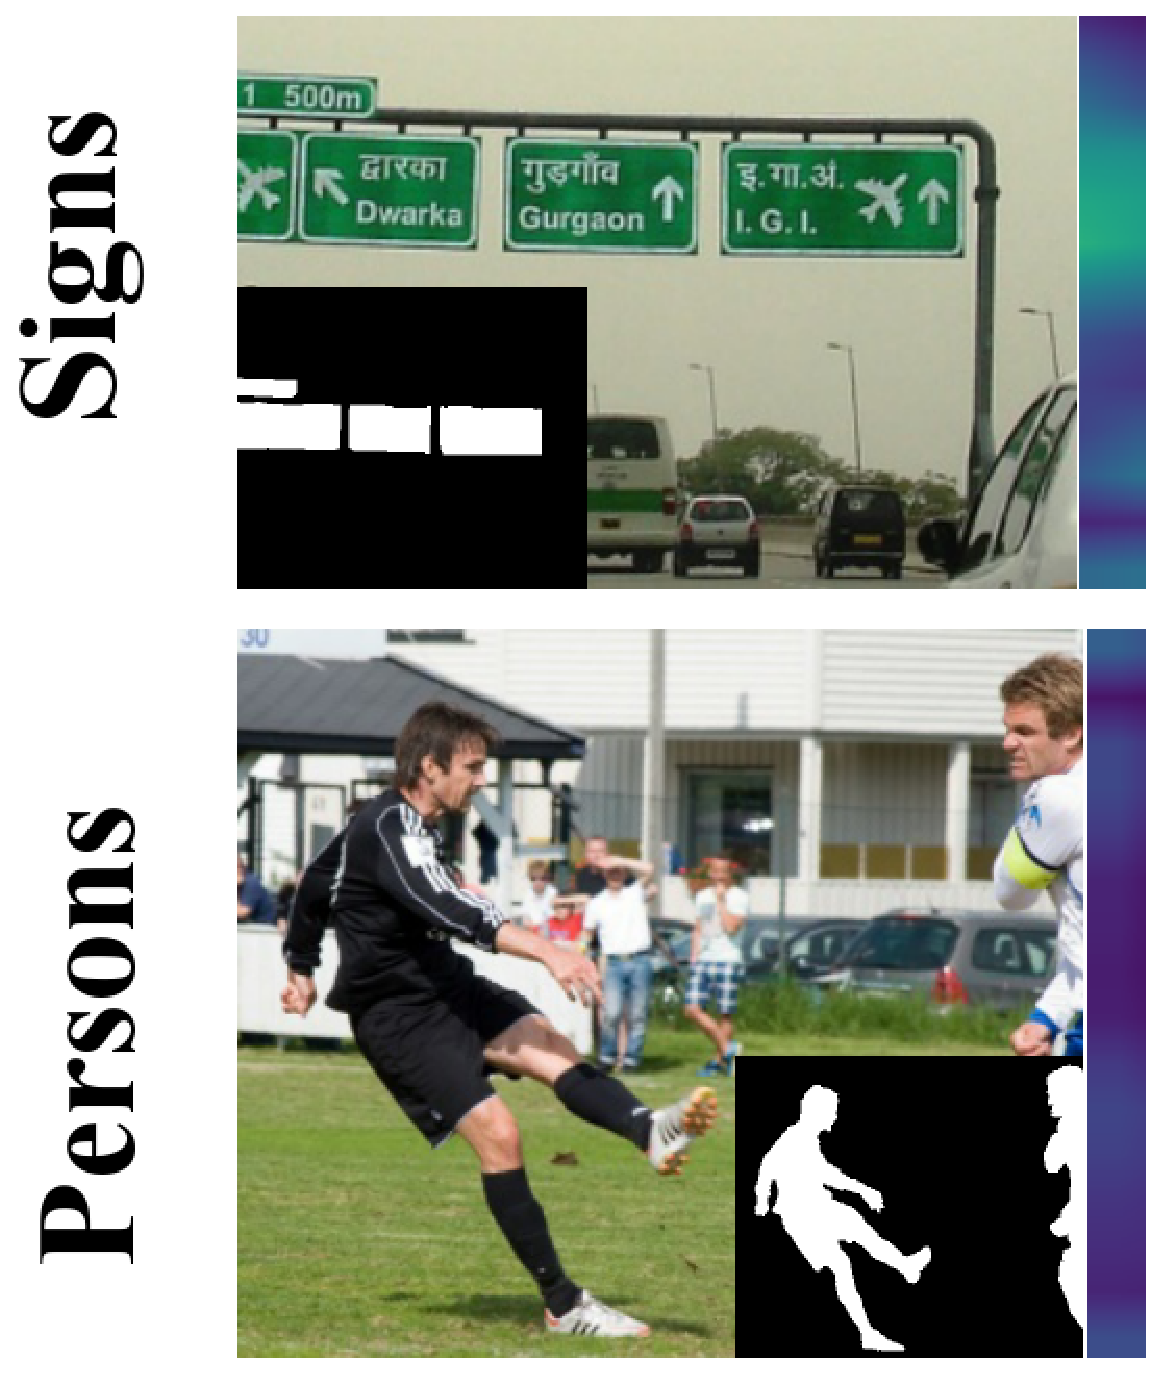
\includegraphics[width=22.94mm,height=27.43mm]{./zengyu_images/image001.eps}

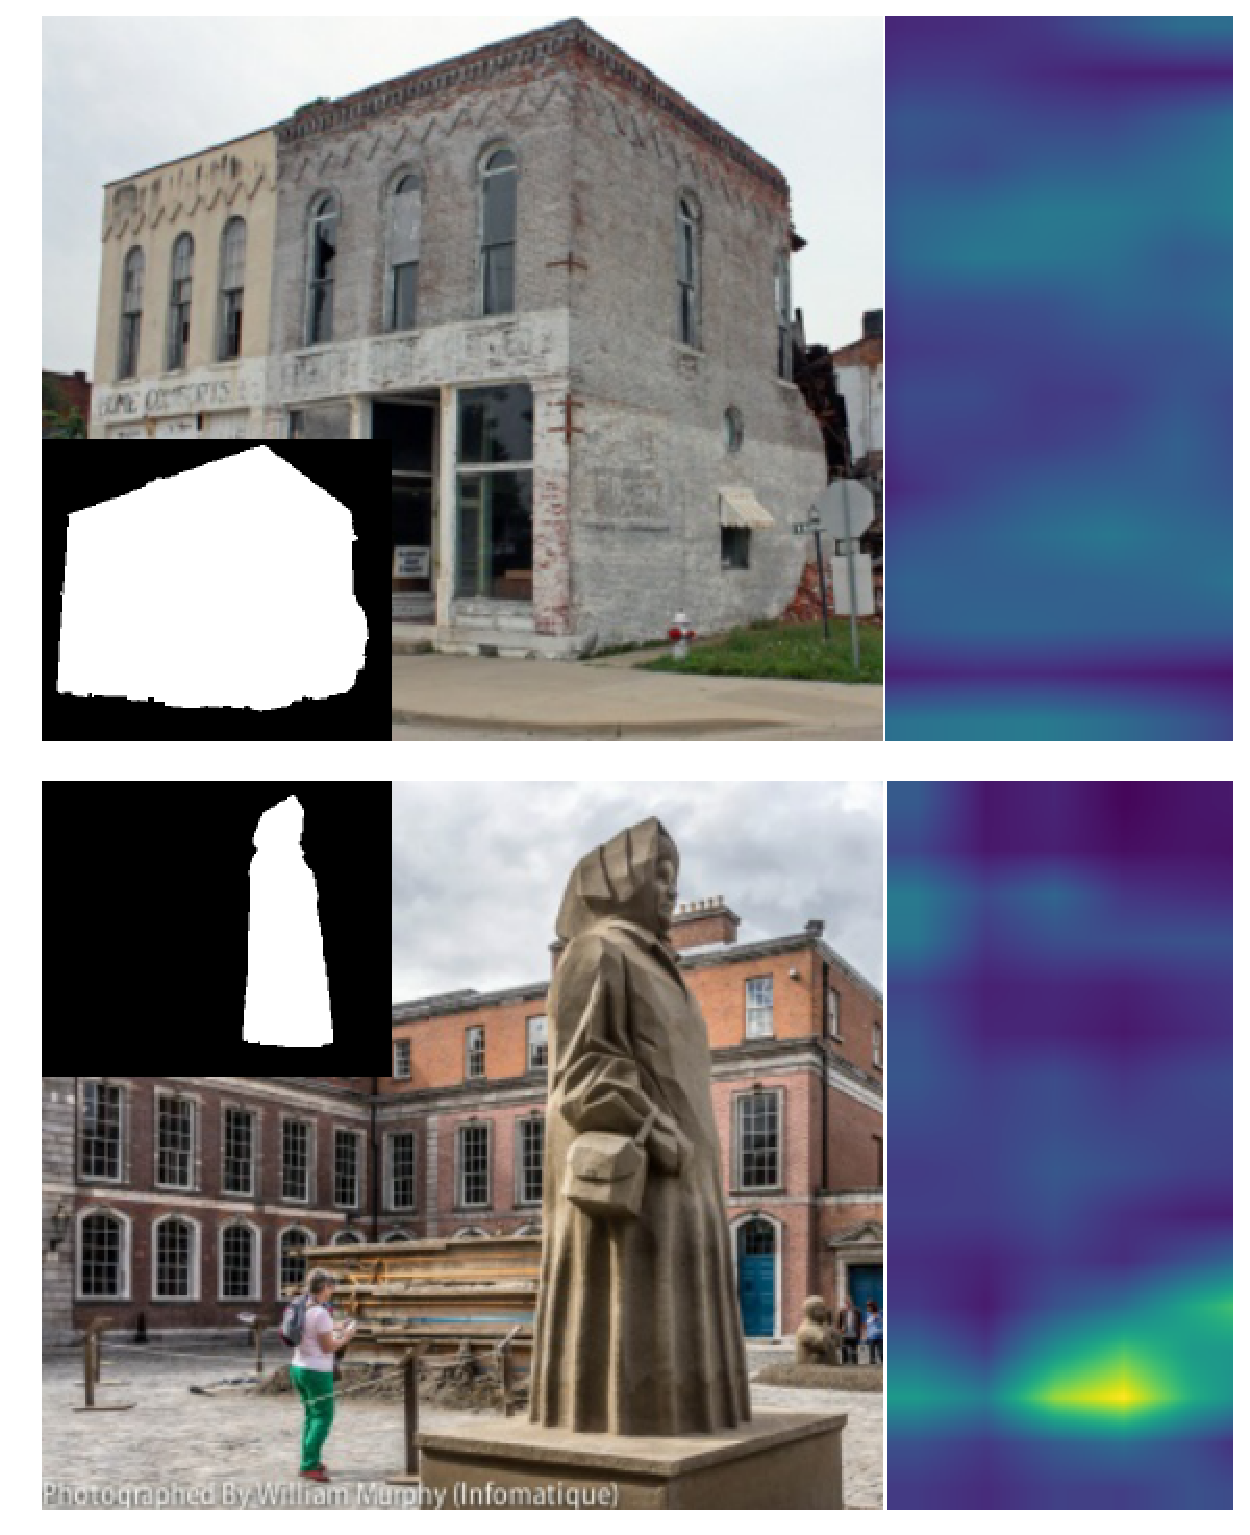
\includegraphics[width=24.72mm,height=30.52mm]{./zengyu_images/image002.eps}
\end{center}
Figure 1. Images and the corresponding feature maps from the last convolution layer of VGG16 $|25|$. The small binary mask in each image indicates the salient object of this image.

networks (DNNs) have been used to remedy the drawbacks of conventional methods. They can learn high-level seman- tic features from training samples, thus are more effective in locating semantically salient regions, yielding more ac- curate results in complex scenes.

DNNs usually need to be trained on a large dataset, while training data for saliency detection is very limited. This is- sue is generally solved by pre-training on a large dataset for other tasks, such as image classification, which easily leads to several problems. First, saliency detection is an image- specific task, and labels should be assigned to pixels de- pending on the image content. However, features produced by pre-trained feature extractors are supposed to work for all images. For example, signs and persons are salient ob- jects in the first column of Figure 1, while they belong to the background in the second column. However, the regions of signs and persons are indiscriminately highlighted in the feature maps in the two columns. With this kind of feature extractor, the prediction model might be enforced to learn to map similar features into opposite labels, which is diffi- cult for small training dataset. Second, categories and ap- pearance of salient objects vary from image to image, while small training data is not enough to capture the diversity. For example, the six salient objects shown in Figure 1 come from six different categories and differ wildly in their ap- pearance. Consequently, it might be hard to learn a unified detector to handle all varieties of salient objects.

Considering the large diversity of salient objects, we avoid training a deep neural network (DNN) that directly maps images into labels. Instead, we train a DNN as an embedding function to map pixels and the attributes of the salient/background regions into a metric space. The at- tributes of the salient/background regions are mapped as anchors in the metric space. Then, a nearest neighbor (NN) classifier is constructed in this space, which assigns each pixel with the label of its nearest anchor. As a non- parametric model, the NN classifier can adapt well to new data and handle the diversity of salient objects. Addition- ally, since the classification task is performed by the NN classifier, the goal of the DNN is turned to learning a gen- eral mapping from the attributes of the salient/background regions to anchors in the embedding space. Compared with directly learning to detect diverse salient objects, this would be easier for the network to learn on limited data.

Concretely, we show the pipeline of our proposed method in Figure 2. During training, the DNN is provided with the true salient and background regions, of which the label of a few randomly selected pixels are flipped, to pro- duce anchors. The output of the NN classifier constitutes a saliency map. The DNN can be trained end-to-end super- vised by the loss between this saliency map and the ground truth. When testing on an image, the saliency map of each image is obtained as in training, but using approximate salient/background regions detected by an existing method. Although the approximate salient/background region is not completely correct, it is often with similar attributes to the true salient/background region. Thus, the corresponding embedding vectors ($i.e$. anchors) would be close to the ones of the true salient/background regions. Further, to produce better results, we propose an iterative testing scheme. The result of the NN classifier is utilized to revise anchors, yield- ing increasingly more accurate results.

Our method can be viewed as a zero-shot learning prob- lem, in which the approximate salient/background regions detected by an existing method provide attributes for unseen salient objects, and the model learns from the training data to learn an image-specific classifier from the attributes to classify pixels of this image. Extensive experiments on five data sets show that our method can significantly improve ac- curacy of existing methods and compares favorably against state-of-the-art approaches.

2. Related works

Generally, saliency detection methods can be catego- rized into two streams: top-down and bottom-up saliency. Since our work addresses bottom-up saliency, here we mainly review recent works on bottom-up saliency, mean- while shortly mention top-down saliency. We also explore the relation between our proposed method and top-down saliency.

Bottom-up (BU) saliency is stimuli-driven, where saliency is derived from contrast among visual stimuli. Conventional bottom-up saliency detection methods often utilize low-level features and heuristic priors. Jiang {\it et al}. $|12|$ formulate saliency detection via an absorbing Markov chain on an image graph model, where saliency of each region is defined as its absorbed time from boundary nodes. Yang {\it et al}. $|32|$ rank the similarity of the image re- gions with foreground cues or background cues via graph- based manifold ranking. Since the conventional methods are not robust in complex scenes neither capable of cap- turing semantic objects, deep neural networks (DNNs) are introduced to overcome these drawbacks. Li {\it et al}. [16] train CNNs with fully connected layers to predict saliency value of each superpixel, and to enhance the spatial coherence of their saliency results using a refinement method. Li {\it et al}. $|18|$ propose a FCN trained under the multi-task learn- ing framework for saliency detection. Zhang {\it et al}. [34] present a generic framework to aggregate multi-level con- volutional features for saliency detection. Although the pro- posed method is also based on DNNs, the main difference between ours and these methods is that they learn a gen- eral model that directly maps images to labels, while our method learns a general embedding function as well as an image-specific NN classifier.

Top-down (TD) saliency aims at finding salient regions specified by a task, and is usually formulated as a super- vised learning problem. Yang and Yang $|33|$ propose a su- pervised top-down saliency model that jointly learns a Con- ditional Random Field (CRF) and a discriminative dictio- nary. Gao {\it et al}. $|9|$ introduced a top-down saliency algo- rithm by selecting discriminant features from a pre-defined filter bank.

Integration of TD and BU saliency has been exploited by some methods. For instance, Borji $|3|$ combines low- level features and saliency maps of previous bottom-up models with top-down cognitive visual features to predict fixations. Tong {\it et al}. $|26|$ proposed a top-down learning approach where the algorithm is bootstrapped with training samples generated using a bottom-up model to exploit the strengths of both bottom-up contrast-based saliency mod- els and top-down learning methods. Our method also can be viewed as an integration of TD and BU saliency. Al- though both our method and the method of Tong {\it et al}. [26] formulate the problem as top-down saliency detection spec- ified by initial saliency maps, there are certain difference between the two. First, Tong's method trains a strong model via boostrap learning with training samples generated by a weak model. In contrast, our method maps pixels and the approximate salient/background regions into a learned met- ric space, which is related to zero-shot learning. Second, thanks to deep learning, our method is capable of captur- ing semantically salient regions and does well on complex
\begin{center}

\includegraphics[width=123.61mm,height=52.15mm]{./zengyu_images/image003.eps}
\end{center}
pixel flow

image flow cross channel $\otimes$ element-wise multiplication   convolution layers

subpixel

$;j\prime\prime\prime$  convolution layers

DNN embeddin $\mathrm{g}$ NN classifier

Figure 2. The pipeline of the proposed method. The input image (a) is first passed through our revised VGG network, resulting in an 512 channel feature map (b) of the same size as the input image. Each pixel is mapped to vectors $e.g.$, (g) and (h) in the learned metric space (j). Salient and background regions is also mapped to vectors . $e$. anchors in the learned metric space. For instance, (e) and (f) are salient and background anchors of this image respectively. During training, the salient and background pixels for producing anchors are selected using a randomly flipped ground truth ((d) and (e) in the figure), see Sec.3.1. An nearest neighbor classifier is built that classifies each pixel based on its distance to the anchors (see Eqn.3 . Classification results of all pixels constitute a saliency map (i), of which loss between the ground truth is used to supervise the network. During testing, the anchors are firstly produced according to an initial saliency map, here (e) is the initial saliency map. Given anchors, the nearest neighbor classifier can produce a new saliency map (i), which is utilized to revise the initial map as in Eqn. 3. Then the revised map is used to produce new approximation to the anchors. Iterating the testing process would result in an increasingly more accurate result.

scenes, while Tong's method uses hand-crafted features and heuristic priors, which are less robust, Third, our method produces pixel-level results, while Tong's method computes saliency value of each image region to assemble a saliency map, which tends to be coarser.

3. The Proposed Method

Our method consists of three components: 1) a DNN as an embedding function {\it i.e}. the anchor network, that maps pixels and regions of the input image into a learned metric space, 2) a nearest neighbor (NN) classifier in the embed- ding space learned specifically for this image to classify its pixels, and 3) an iterative testing scheme that utilizes the result of the NN classifier to revise anchors, yielding in- creasingly more accurate results.

3.1. The anchor network

Let $x_{mn}$ denote a pixel of an image $X_{m}$. Each im- age consists a salient and a background region, . $e. X_{m}= C_{m1}\cup C_{m2}$. Each pixel of an image either belongs to salient or background regions, denoted as $n\in C_{mk}, k=1$, 2, re- spectively. We use an embedding function modeled by a DNN $\phi$ with parameter $\theta$, to map each pixel to a vector in a $\mathrm{D}$-dimensional space:
\begin{center}
$\phi_{mn}=\phi(x_{mn};\theta)$ ,   (1)
\end{center}
where $\phi_{mn}$ is the embedding vector to the corresponding pixel $x_{mn}.$

The salient or background region $C_{mk}$ is also mapped into vectors in $D$-dimensional metric space by a DNN $\psi$ with parameter $\eta$:
\begin{center}
$\mu_{mk}=\psi(C_{mk};\eta)$ ,   (2)
\end{center}
in which $\mu_{mk}$ is the mapping of the salient or background region, . $e$. anchors.

We assume that in the embedding space, all pixels of an image cluster around the corresponding anchors of this im- age. Then a nearest neighbor classifier can be built specif- ically for this image by classifying each pixel according to its nearest anchor. The probability of a pixel $x_{mn}$ of image $X_{m}$ belonging to $C_{mk}$ can be given by the softmax over its distance to the anchors:
\begin{center}
$p(C_{mk}|x_{mn})=\displaystyle \frac{\exp\{-d(\phi_{mn},\mu_{mk})\}}{\sum_{j}\exp\{-d(\phi_{mn},\mu_{mj})\}}$,   (3)
\end{center}
where $\phi_{mn}$ and $\mu_{mk}$ are the vectors of pixel $x_{mn}$ and the salien$\mathrm{t}/$ backgro und anchor given by Eqn.1 and 2. $d()$ de- notes Euclidean distance.

The CNN embeddings can be trained using a gradient- based optimization algorithm through maximizing the $\log$ likelihood with respect to $\theta$ and $\eta$ on the training set:

$\displaystyle \mathcal{L}=\sum_{m,n}t_{mn}\log p(C_{m1}|x_{mn})+(1-t_{mn})\log p(C_{m2}|x_{mn})$ , (4) where $t_{mn}$ is the label of pixel $x_{mn}. t_{mn}=1$ when $x_{mn}\in C_{1}$, {\it i.e}. salient and $t_{mn}=0$ when $x_{mn}\in C_{2}$, {\it i.e}. background.

In practice, the ground-truth will not be available dur- ing testing, and the anchors are produced according to a prior saliency map, which is inaccurate. Therefore, to match training and testing conditions, during training we randomly flip the label of each pixel with probability $p$ when pro- ducing the anchors using Eqn.2. In addition, this random

flipping also increases diversity of training samples, thus helping reduce overfitting. We explain the training process of the anchor network in Alg. 1. Here, $\mathcal{L}_{m}$ denotes the $\log$ likelihood on the image $X_{m}.$

Algorithm1: Training the anchor network.

Input:Training set $\{(X_{m}, t_{m}$

in which $t_{mn}=1$ indicates $x_{mn}\in C_{m1},$ and $t_{mn}=0$ otherwise.

Out put: CN$\mathrm{N}$ embedding $\phi \theta$) and $\psi \eta$)

1 for {\it training iterations} do

2

Sample a pair of training image and ground truth map $(X_{m},\ t_{m}\ )$ from the train ing set.

3

Randomly flip the elements in $t_{m}$ with probability
$$
p.
$$
4

Compute the embedding vector $\phi_{mn}$ of each pixel given by Eqn.1 and produce anchors $\mu_{mk}$ as in Eqn.2.

5

Compute gradient of $\log$ likelihood $\mathcal{L}_{m}$ on this

image with respect to $\theta$ and $\eta.$

6

Update $\theta$ and $\eta$ according to $\nabla_{\theta,\eta}\mathcal{L}_{m}$ using a

gradient based optimization method.

7 end

3.2. Iterative testing scheme

In the testing phase, since the ground-truth is unknown, it is not possible to obtain precise salient and background re- gions to produce anchors as in the training time. Therefore, we produce anchors using approximate salient/background regions $\hat{C}_{mk}$ selected according to the saliency map $Y_{m}^{(0)}$ of an existing method. An iterative testing scheme is proposed to gradually revise the anchors using the result of the NN classifier.

In the t-th iteration $(t>0)$ , the anchors are generated according to salient/background region $\hat{C}_{mk}$ selected by the prior saliency map $Y_{m}^{(t)}$. Given the anchors, we use the near- est neighbor classifier as in Eqn.3 to compute the probabil- ity of each pixel belonging to salient regions, . $e$. saliency value, constructing another saliency map $Z_{m}^{(t)}$. Then, the prior saliency map is updated with

$Y_{m}^{(t+1)}=\displaystyle \frac{t}{t+1}Y_{m}^{(t)}+\frac{1}{t+1}Z_{m}^{(t)}$, (5)

where $Y_{m}^{(t+1)}$ is the prior saliency map which will be used for selecting salient and background regions in the next it-

flipping also increases diversity of training samples, thus helping reduce overfitting. We explain the training process of the anchor network in Alg. 1. Here, $\mathcal{L}_{m}$ denotes the $\log$ likelihood on the image $X_{m}.$

Algorithm1: Training the anchor network.

Input:Training set $\{(X_{m}, t_{m}$

in which $t_{mn}=1$ indicates $x_{mn}\in C_{m1},$ and $t_{mn}=0$ otherwise.

Out put: CN$\mathrm{N}$ embedding $\phi \theta$) and $\psi \eta$)

1 for {\it training iterations} do

2

Sample a pair of training image and ground truth map $(X_{m},\ t_{m}\ )$ from the train ing set.

3

Randomly flip the elements in $t_{m}$ with probability
$$
p.
$$
4

Compute the embedding vector $\phi_{mn}$ of each pixel given by Eqn.1 and produce anchors $\mu_{mk}$ as in Eqn.2.

5

Compute gradient of $\log$ likelihood $\mathcal{L}_{m}$ on this

image with respect to $\theta$ and $\eta.$

6

Update $\theta$ and $\eta$ according to $\nabla_{\theta,\eta}\mathcal{L}_{m}$ using a

gradient based optimization method.

7 end

3.2. Iterative testing scheme

In the testing phase, since the ground-truth is unknown, it is not possible to obtain precise salient and background re- gions to produce anchors as in the training time. Therefore, we produce anchors using approximate salient/background regions $\hat{C}_{mk}$ selected according to the saliency map $Y_{m}^{(0)}$ of an existing method. An iterative testing scheme is proposed to gradually revise the anchors using the result of the NN classifier.

In the t-th iteration $(t>0)$ , the anchors are generated according to salient/background region $\hat{C}_{mk}$ selected by the prior saliency map $Y_{m}^{(t)}$. Given the anchors, we use the near- est neighbor classifier as in Eqn.3 to compute the probabil- ity of each pixel belonging to salient regions, . $e$. saliency value, constructing another saliency map $Z_{m}^{(t)}$. Then, the prior saliency map is updated with

$Y_{m}^{(t+1)}=\displaystyle \frac{t}{t+1}Y_{m}^{(t)}+\frac{1}{t+1}Z_{m}^{(t)}$, (5)

where $Y_{m}^{(t+1)}$ is the prior saliency map which will be used for selecting salient and background regions in the next it-

flipping also increases diversity of training samples, thus helping reduce overfitting. We explain the training process of the anchor network in Alg. 1. Here, $\mathcal{L}_{m}$ denotes the $\log$ likelihood on the image $X_{m}.$

Algorithm1: Training the anchor network.

Input:Training set $\{(X_{m}, t_{m}$

in which $t_{mn}=1$ indicates $x_{mn}\in C_{m1},$ and $t_{mn}=0$ otherwise.

Out put: CN$\mathrm{N}$ embedding $\phi \theta$) and $\psi \eta$)

1 for {\it training iterations} do

2

Sample a pair of training image and ground truth map $(X_{m},\ t_{m}\ )$ from the train ing set.

3

Randomly flip the elements in $t_{m}$ with probability
$$
p.
$$
4

Compute the embedding vector $\phi_{mn}$ of each pixel given by Eqn.1 and produce anchors $\mu_{mk}$ as in Eqn.2.

5

Compute gradient of $\log$ likelihood $\mathcal{L}_{m}$ on this

image with respect to $\theta$ and $\eta.$

6

Update $\theta$ and $\eta$ according to $\nabla_{\theta,\eta}\mathcal{L}_{m}$ using a

gradient based optimization method.

7 end

3.2. Iterative testing scheme

In the testing phase, since the ground-truth is unknown, it is not possible to obtain precise salient and background re- gions to produce anchors as in the training time. Therefore, we produce anchors using approximate salient/background regions $\hat{C}_{mk}$ selected according to the saliency map $Y_{m}^{(0)}$ of an existing method. An iterative testing scheme is proposed to gradually revise the anchors using the result of the NN classifier.

In the t-th iteration $(t>0)$ , the anchors are generated according to salient/background region $\hat{C}_{mk}$ selected by the prior saliency map $Y_{m}^{(t)}$. Given the anchors, we use the near- est neighbor classifier as in Eqn.3 to compute the probabil- ity of each pixel belonging to salient regions, . $e$. saliency value, constructing another saliency map $Z_{m}^{(t)}$. Then, the prior saliency map is updated with

$Y_{m}^{(t+1)}=\displaystyle \frac{t}{t+1}Y_{m}^{(t)}+\frac{1}{t+1}Z_{m}^{(t)}$, (5)

where $Y_{m}^{(t+1)}$ is the prior saliency map which will be used for selecting salient and background regions in the next it-

flipping also increases diversity of training samples, thus helping reduce overfitting. We explain the training process of the anchor network in Alg. 1. Here, $\mathcal{L}_{m}$ denotes the $\log$ likelihood on the image $X_{m}.$

Algorithm1: Training the anchor network.

Input:Training set $\{(X_{m}, t_{m}$

in which $t_{mn}=1$ indicates $x_{mn}\in C_{m1},$ and $t_{mn}=0$ otherwise.

Out put: CN$\mathrm{N}$ embedding $\phi \theta$) and $\psi \eta$)

1 for {\it training iterations} do

2

Sample a pair of training image and ground truth map $(X_{m},\ t_{m}\ )$ from the train ing set.

3

Randomly flip the elements in $t_{m}$ with probability
$$
p.
$$
4

Compute the embedding vector $\phi_{mn}$ of each pixel given by Eqn.1 and produce anchors $\mu_{mk}$ as in Eqn.2.

5

Compute gradient of $\log$ likelihood $\mathcal{L}_{m}$ on this

image with respect to $\theta$ and $\eta.$

6

Update $\theta$ and $\eta$ according to $\nabla_{\theta,\eta}\mathcal{L}_{m}$ using a

gradient based optimization method.

7 end

3.2. Iterative testing scheme

In the testing phase, since the ground-truth is unknown, it is not possible to obtain precise salient and background re- gions to produce anchors as in the training time. Therefore, we produce anchors using approximate salient/background regions $\hat{C}_{mk}$ selected according to the saliency map $Y_{m}^{(0)}$ of an existing method. An iterative testing scheme is proposed to gradually revise the anchors using the result of the NN classifier.

In the t-th iteration $(t>0)$ , the anchors are generated according to salient/background region $\hat{C}_{mk}$ selected by the prior saliency map $Y_{m}^{(t)}$. Given the anchors, we use the near- est neighbor classifier as in Eqn.3 to compute the probabil- ity of each pixel belonging to salient regions, . $e$. saliency value, constructing another saliency map $Z_{m}^{(t)}$. Then, the prior saliency map is updated with

$Y_{m}^{(t+1)}=\displaystyle \frac{t}{t+1}Y_{m}^{(t)}+\frac{1}{t+1}Z_{m}^{(t)}$, (5)

where $Y_{m}^{(t+1)}$ is the prior saliency map which will be used for selecting salient and background regions in the next it-

flipping also increases diversity of training samples, thus helping reduce overfitting. We explain the training process of the anchor network in Alg. 1. Here, $\mathcal{L}_{m}$ denotes the $\log$ likelihood on the image $X_{m}.$

Algorithm1: Training the anchor network.

Input:Training set $\{(X_{m}, t_{m}$

in which $t_{mn}=1$ indicates $x_{mn}\in C_{m1},$ and $t_{mn}=0$ otherwise.

Out put: CN$\mathrm{N}$ embedding $\phi \theta$) and $\psi \eta$)

1 for {\it training iterations} do

2

Sample a pair of training image and ground truth map $(X_{m},\ t_{m}\ )$ from the train ing set.

3

Randomly flip the elements in $t_{m}$ with probability
$$
p.
$$
4

Compute the embedding vector $\phi_{mn}$ of each pixel given by Eqn.1 and produce anchors $\mu_{mk}$ as in Eqn. 2.

5

Compute gradient of $\log$ likelihood $\mathcal{L}_{m}$ on this

image with respect to $\theta$ and $\eta.$

6

Update $\theta$ and $\eta$ according to $\nabla_{\theta,\eta}\mathcal{L}_{m}$ using a

gradient based optimization method.

7 end

3.2. Iterative testing scheme

In the testing phase, since the ground-truth is unknown, it is not possible to obtain precise salient and background re- gions to produce anchors as in the training time. Therefore, we produce anchors using approximate salient/background regions $\hat{C}_{mk}$ selected according to the saliency map $Y_{m}^{(0)}$ of an existing method. An iterative testing scheme is proposed to gradually revise the anchors using the result of the NN classifier.

In the t-th iteration $(t>0)$ , the anchors are generated according to salient/background region $\hat{C}_{mk}$ selected by the prior saliency map $Y_{m}^{(t)}$. Given the anchors, we use the near- est neighbor classifier as in Eqn.3 to compute the probabil- ity of each pixel belonging to salient regions, . $e$. saliency value, constructing another saliency map $Z_{m}^{(t)}$. Then, the prior saliency map is updated with

$Y_{m}^{(t+1)}=\displaystyle \frac{t}{t+1}Y_{m}^{(t)}+\frac{1}{t+1}Z_{m}^{(t)}$, (5)

where $Y_{m}^{(t+1)}$ is the prior saliency map which will be used for selecting salient and background regions in the next it-

flipping also increases diversity of training samples, thus helping reduce overfitting. We explain the training process of the anchor network in Alg. 1. Here, $\mathcal{L}_{m}$ denotes the $\log$ likelihood on the image $X_{m}.$

Algorithm1: Training the anchor network.

Input:Training set $\{(X_{m}, t_{m}$

in which $t_{mn}=1$ indicates $x_{mn}\in C_{m1},$ and $t_{mn}=0$ otherwise.

Out put: CN$\mathrm{N}$ embedding $\phi \theta$) and $\psi \eta$)

1 for {\it training iterations} do

2

Sample a pair of training image and ground truth map $(X_{m},\ t_{m}\ )$ from the train ing set.

3

Randomly flip the elements in $t_{m}$ with probability
$$
p.
$$
4

Compute the embedding vector $\phi_{mn}$ of each pixel given by Eqn.1 and produce anchors $\mu_{mk}$ as in Eqn.2.

5

Compute gradient of $\log$ likelihood $\mathcal{L}_{m}$ on this

image with respect to $\theta$ and $\eta.$

6

Update $\theta$ and $\eta$ according to $\nabla_{\theta,\eta}\mathcal{L}_{m}$ using a

gradient based optimization method.

7 end

3.2. Iterative testing scheme

In the testing phase, since the ground-truth is unknown, it is not possible to obtain precise salient and background re- gions to produce anchors as in the training time. Therefore, we produce anchors using approximate salient/background regions $\hat{C}_{mk}$ selected according to the saliency map $Y_{m}^{(0)}$ of an existing method. An iterative testing scheme is proposed to gradually revise the anchors using the result of the NN classifier.

In the t-th iteration $(t>0)$ , the anchors are generated according to salient/background region $\hat{C}_{mk}$ selected by the prior saliency map $Y_{m}^{(t)}$. Given the anchors, we use the near- est neighbor classifier as in Eqn.3 to compute the probabil- ity of each pixel belonging to salient regions, . $e$. saliency value, constructing another saliency map $Z_{m}^{(t)}$. Then, the prior saliency map is updated with

$Y_{m}^{(t+1)}=\displaystyle \frac{t}{t+1}Y_{m}^{(t)}+\frac{1}{t+1}Z_{m}^{(t)}$, (5)

where $Y_{m}^{(t+1)}$ is the prior saliency map which will be used for selecting salient and background regions in the next it-

flipping also increases diversity of training samples, thus helping reduce overfitting. We explain the training process of the anchor network in Alg. 1. Here, $\mathcal{L}_{m}$ denotes the $\log$ likelihood on the image $X_{m}.$

Algorithm1: Training the anchor network.

Input:Training set $\{(X_{m}, t_{m}$

in which $t_{mn}=1$ indicates $x_{mn}\in C_{m1},$ and $t_{mn}=0$ otherwise.

Out put: CN$\mathrm{N}$ embedding $\phi \theta$) and $\psi \eta$)

1 for {\it training iterations} do

2

Sample a pair of training image and ground truth map $(X_{m},\ t_{m}\ )$ from the train ing set.

3

Randomly flip the elements in $t_{m}$ with probability
$$
p.
$$
4

Compute the embedding vector $\phi_{mn}$ of each pixel given by Eqn.1 and produce anchors $\mu_{mk}$ as in Eqn. 2.

5

Compute gradient of $\log$ likelihood $\mathcal{L}_{m}$ on this

image with respect to $\theta$ and $\eta.$

6

Update $\theta$ and $\eta$ according to $\nabla_{\theta,\eta}\mathcal{L}_{m}$ using a

gradient based optimization method.

7 end

3.2. Iterative testing scheme

In the testing phase, since the ground-truth is unknown, it is not possible to obtain precise salient and background re- gions to produce anchors as in the training time. Therefore, we produce anchors using approximate salient/background regions $\hat{C}_{mk}$ selected according to the saliency map $Y_{m}^{(0)}$ of an existing method. An iterative testing scheme is proposed to gradually revise the anchors using the result of the NN classifier.

In the t-th iteration $(t>0)$ , the anchors are generated according to salient/background region $\hat{C}_{mk}$ selected by the prior saliency map $Y_{m}^{(t)}$. Given the anchors, we use the near- est neighbor classifier as in Eqn.3 to compute the probabil- ity of each pixel belonging to salient regions, . $e$. saliency value, constructing another saliency map $Z_{m}^{(t)}$. Then, the prior saliency map is updated with

$Y_{m}^{(t+1)}=\displaystyle \frac{t}{t+1}Y_{m}^{(t)}+\frac{1}{t+1}Z_{m}^{(t)}$, (5)

where $Y_{m}^{(t+1)}$ is the prior saliency map which will be used for selecting salient and background regions in the next it-

flipping also increases diversity of training samples, thus helping reduce overfitting. We explain the training process of the anchor network in Alg. 1. Here, $\mathcal{L}_{m}$ denotes the $\log$ likelihood on the image $X_{m}.$

Algorithm1: Training the anchor network.

Input:Training set $\{(X_{m}, t_{m}$

in which $t_{mn}=1$ indicates $x_{mn}\in C_{m1},$ and $t_{mn}=0$ otherwise.

Out put: CN$\mathrm{N}$ embedding $\phi \theta$) and $\psi \eta$)

1 for {\it training iterations} do

2

Sample a pair of training image and ground truth map $(X_{m},\ t_{m}\ )$ from the train ing set.

3

Randomly flip the elements in $t_{m}$ with probability
$$
p.
$$
4

Compute the embedding vector $\phi_{mn}$ of each pixel given by Eqn.1 and produce anchors $\mu_{mk}$ as in Eqn.2.

5

Compute gradient of $\log$ likelihood $\mathcal{L}_{m}$ on this

image with respect to $\theta$ and $\eta.$

6

Update $\theta$ and $\eta$ according to $\nabla_{\theta,\eta}\mathcal{L}_{m}$ using a

gradient based optimization method.

7 end

3.2. Iterative testing scheme

In the testing phase, since the ground-truth is unknown, it is not possible to obtain precise salient and background re- gions to produce anchors as in the training time. Therefore, we produce anchors using approximate salient/background regions $\hat{C}_{mk}$ selected according to the saliency map $Y_{m}^{(0)}$ of an existing method. An iterative testing scheme is proposed to gradually revise the anchors using the result of the NN classifier.

In the t-th iteration $(t>0)$ , the anchors are generated according to salient/background region $\hat{C}_{mk}$ selected by the prior saliency map $Y_{m}^{(t)}$. Given the anchors, we use the near- est neighbor classifier as in Eqn.3 to compute the probabil- ity of each pixel belonging to salient regions, . $e$. saliency value, constructing another saliency map $Z_{m}^{(t)}$. Then, the prior saliency map is updated with

$Y_{m}^{(t+1)}=\displaystyle \frac{t}{t+1}Y_{m}^{(t)}+\frac{1}{t+1}Z_{m}^{(t)}$, (5)

where $Y_{m}^{(t+1)}$ is the prior saliency map which will be used for selecting salient and background regions in the next it-

Figure 3 shows the process of the initial maps being promoted by the proposed method. Although the initial saliency map may not precisely separate the foreground and background, it can often partially separate them, and thus can provide information regarding categories and appear- ance of salient objects in the image. For instance, in the first image of Figure 3, though only a small part of the foreground is highlighted, the initial map can tell us that the foreground may be a gorilla, and the background con- tains a piece of green. Then, its selected foreground/back- ground regions should be similar to the true foreground/ background regions, leading to the corresponding anchors close to the true ones in the learned metric space. Thereby the nearest neighbor classification given by Eqn.3 can pro- duce a good result. As the iterations progress, the approx- imate anchors gradually approach to the true ones, which would result in a better result. This, in turn could provide an increasingly accurate approximation to the anchors, and thus a more accurate result. As shown in Figure 3, the ini- tial maps are not appealing, while the modified maps by our method look much better.

Algorithm2:Testing algorithm of the proposed method.  Input:The input image $X$, the initial saliency map $Y^{(0)}$, the number of iterations $T.$

Output: The promoted saliency map $Y^{(T)}.$

1 Compute th $\mathrm{e}$ embedding vector $\phi_{n}$ of each pixel $x_{n}$

of {\it X}. for $t\in\{1,\ T\}$ do

2

Select the approximate salient $C_{1}$ and background region $C_{2}$ according to $Y^{(t)}.$

3 Produce the approximate anchor
$$
\hat{\mu}_{k}=\psi(C_{k};\eta)\ ,\ k=1,\ 2.
$$
4

Compute saliency value of each pixel according to Eqn.3 to constitute another saliency map $Z_{m}^{(t)}.$ 5

Update the prior saliency map:
$$
Y^{(t+1)}\leftarrow\frac{t}{t+1}Y^{(t)}+\frac{1}{t+1}Z^{(t)}
$$
6 end

It is known that DNNs, which typically consist of many parameters, have to be trained on large datasets to obtain good performance. For tasks where training data is scarce, such as saliency detection, revising a DNN that has been pre-trained on image classification datasets is the most vi- able option. Therefore, we also adopt a pre-trained DNN for our purpose rather than training a DNN from scratch. We modify the VGG16 $|25|$ network, pre-trained on the Im-

eration. This means that the prior map is updated to a weighted sum of itself and the new result. After the first iteration, the prior map is completely replaced by the new result. The weight of the new result decreases with iterating, which insures stability of the iteration process. The testing algorithm of the proposed method is shown in Alg.2.
\begin{center}
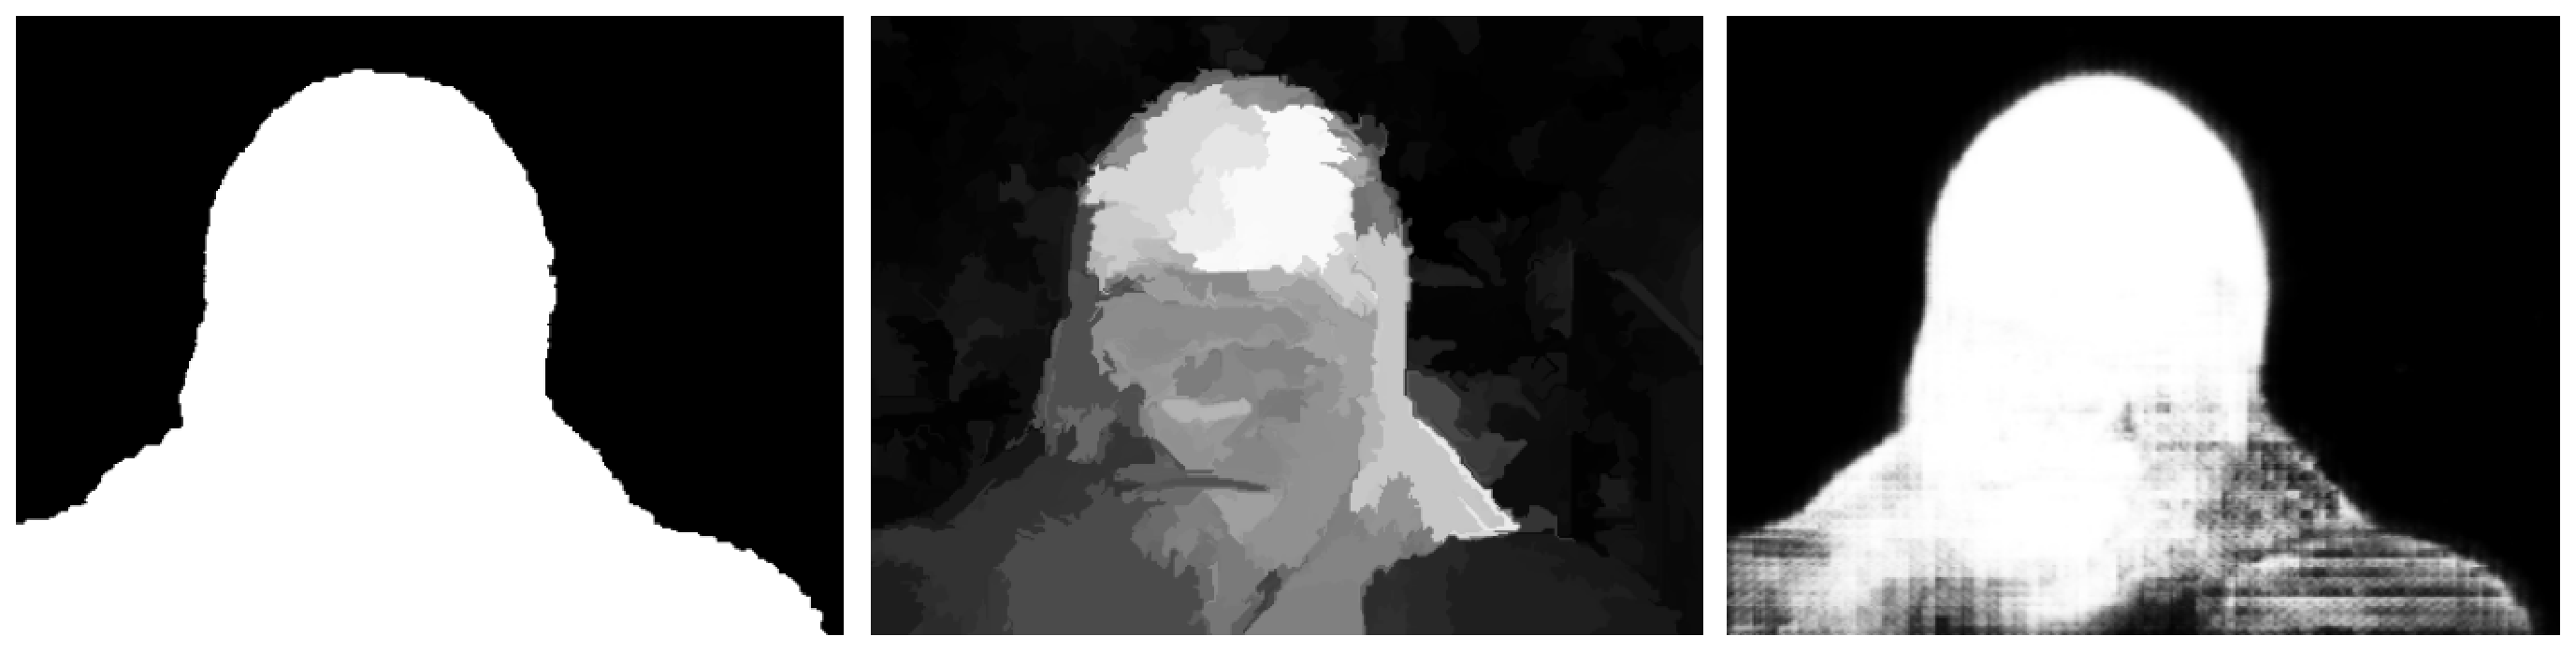
\includegraphics[width=55.29mm,height=13.46mm]{./zengyu_images/image004.eps}

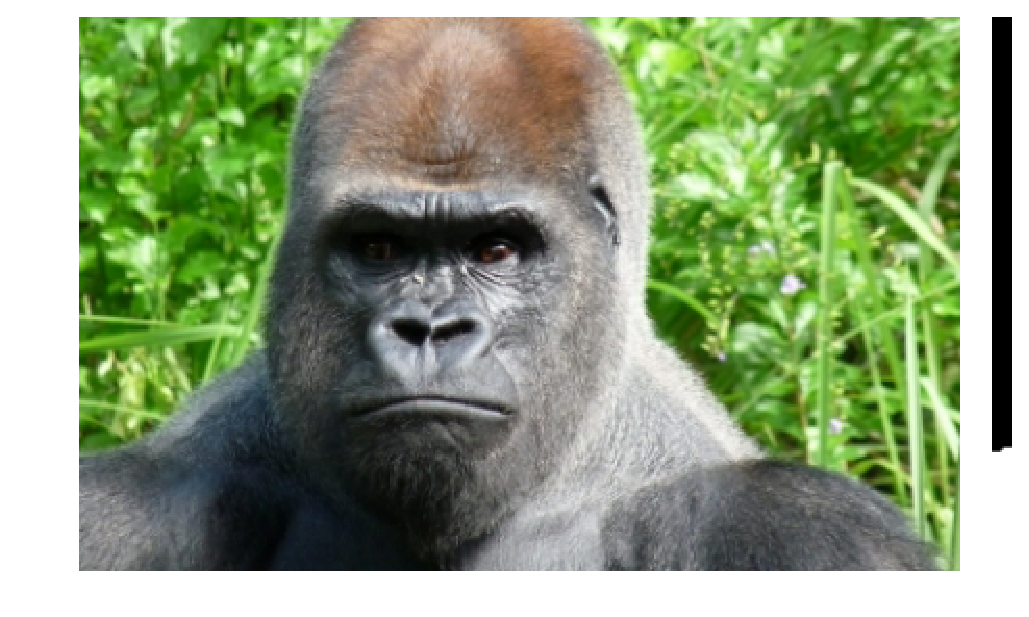
\includegraphics[width=20.24mm,height=11.85mm]{./zengyu_images/image005.eps}

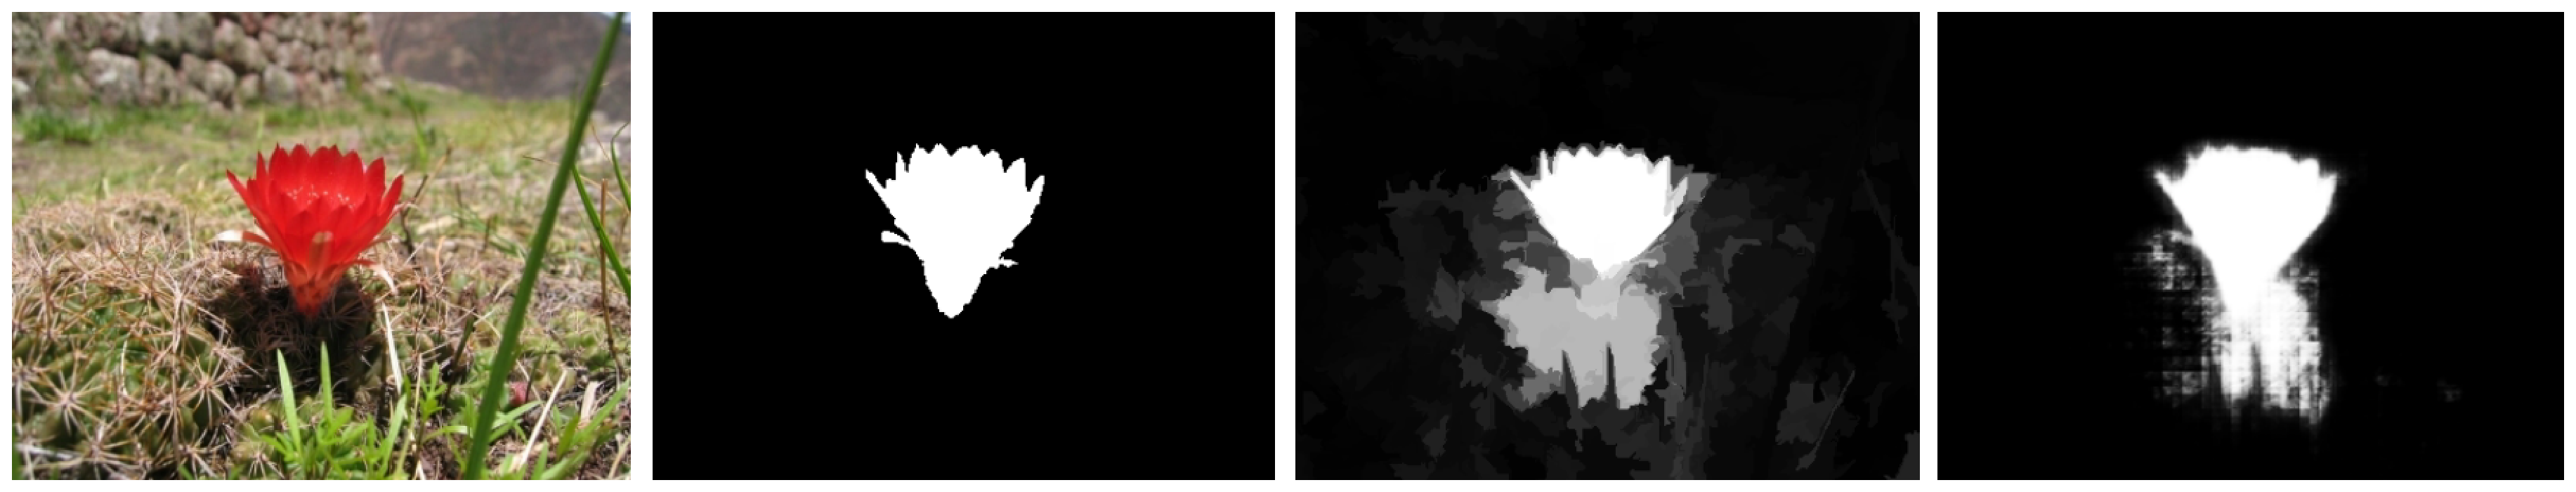
\includegraphics[width=73.83mm,height=13.55mm]{./zengyu_images/image006.eps}
\end{center}
Image GT $\mathrm{t}=0 \mathrm{t}=1$
\begin{center}
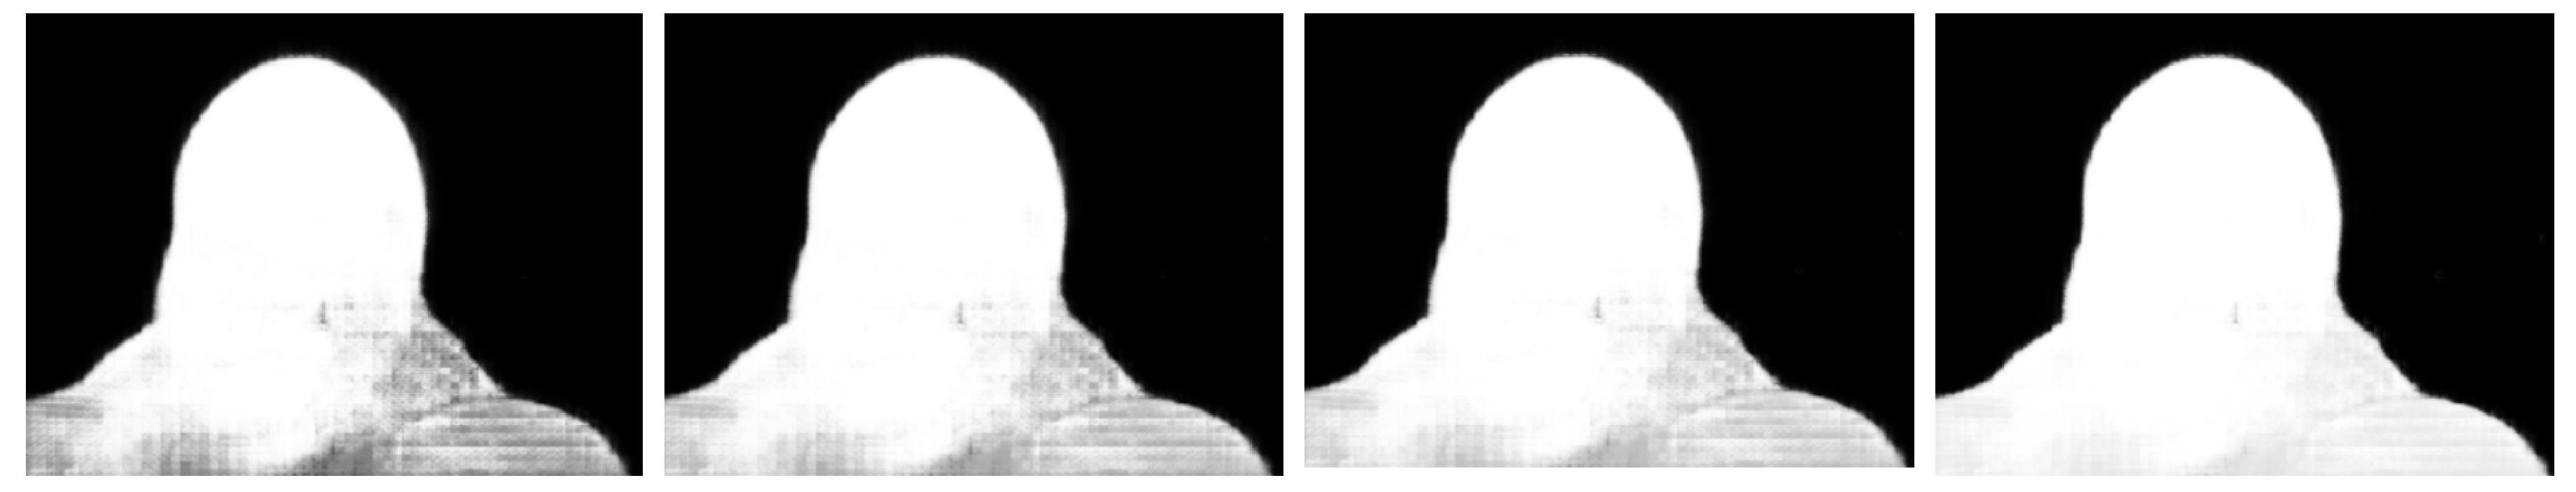
\includegraphics[width=74.17mm,height=13.63mm]{./zengyu_images/image007.eps}

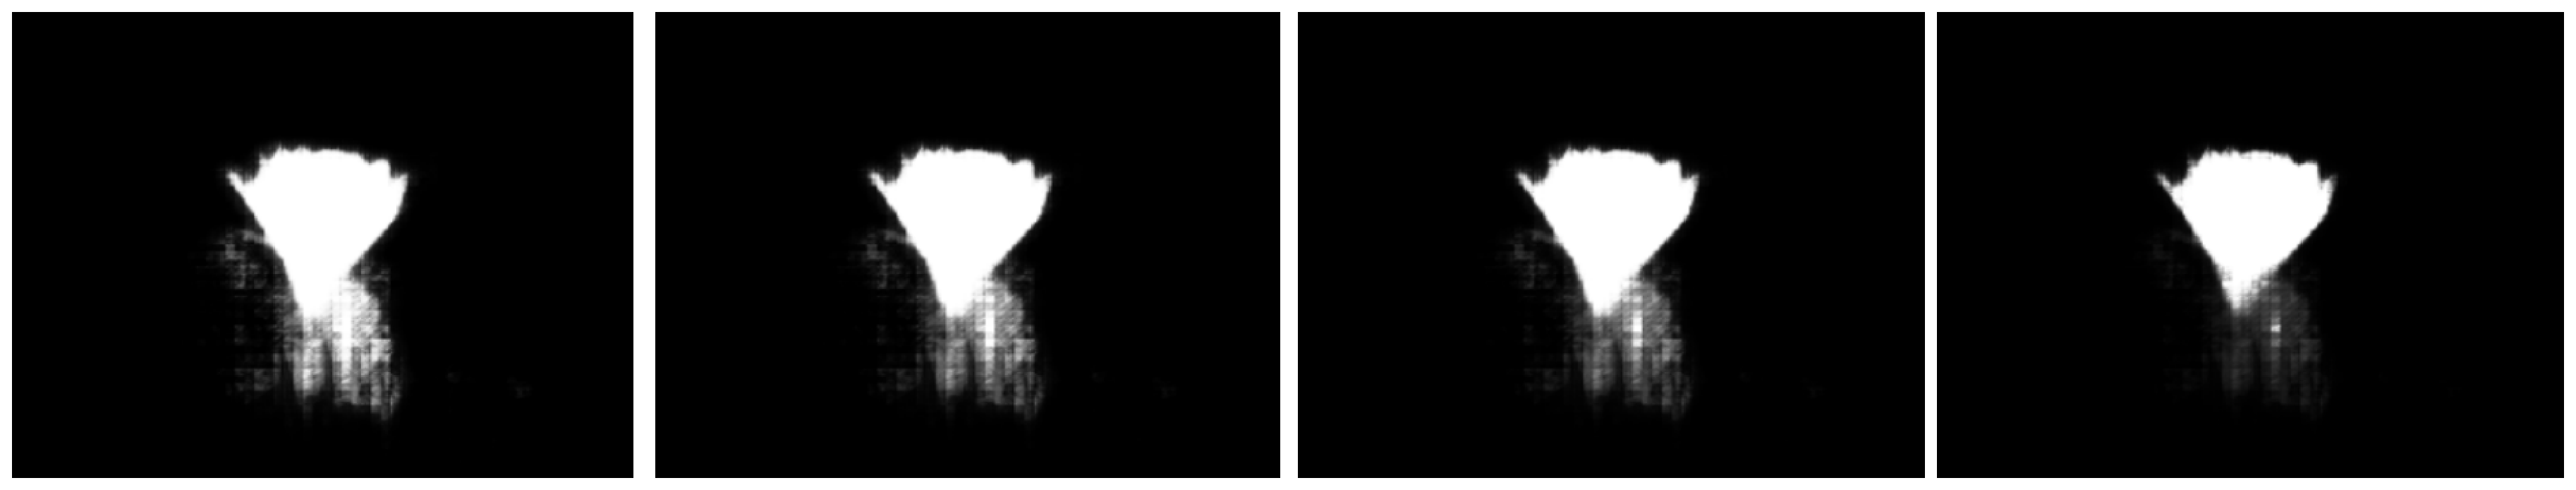
\includegraphics[width=73.53mm,height=13.42mm]{./zengyu_images/image008.eps}
$$
\mathrm{t}=2\ \mathrm{t}=3\ \mathrm{t}=4\ \mathrm{t}=10
$$
\end{center}
Figure 3. The process of the initial maps being promoted by the proposed method.

ageNet [7] dataset, into the pixe 1 embedding $\phi \theta$) and region embeddin $\mathrm{g}\psi (\ \eta)$ . Sin ce the D NN serves as an em- bedding instead of a classifier in the proposed method, we remove all the fully connected layers of VGG, and only re- tain its feature extractor component (VGG feature extrac- tor). The VGG feature extractor consists of 5 convolution blocks, each of which contains several convolution and non- linear layers, as well as a pooling layer. We show the net- work architecture and the overall structure of the proposed method in Figure 2, and describe the details in the next two subsections. In the figures and the text of this section, nonlinearity layers and batch-normalization layers are omit to avoid clutter. The combination of a convolution$/$fully connected layer, a batch-normalization layer and a ReLU nonlinear Convolution layers are referred to as a convolu- tion fully connected layers in this section.

3.3. Pixel embedding

Although effective in extracting hierarchical features, VGG feature extractor makes the feature maps smaller than the input image. This is not desirable for our method, be- cause in order to map each pixel of the input image to a vector in the learned metric space, the embedding CNN should produce feature maps of the same resolution as the input image. We adopt two strategies to obtain larger feature maps: 1) remove the pooling layers of the last two convo- lution blocks and use dilated convolutions in these blocks to maintain receptive filed of the convolution filters, and 2) append a subpixel convolution layer after each convolution block of the VGG feature extractor to upsample the feature maps of each convolution blocks to the input image size. Subpixel convolution is an upsampling strategy originally proposed in [24] for image super-resolution. To produce a $C$-channel tensor of $N$ times the input size, the subpixel convolution firstly performs convolution on the feature map
\begin{center}
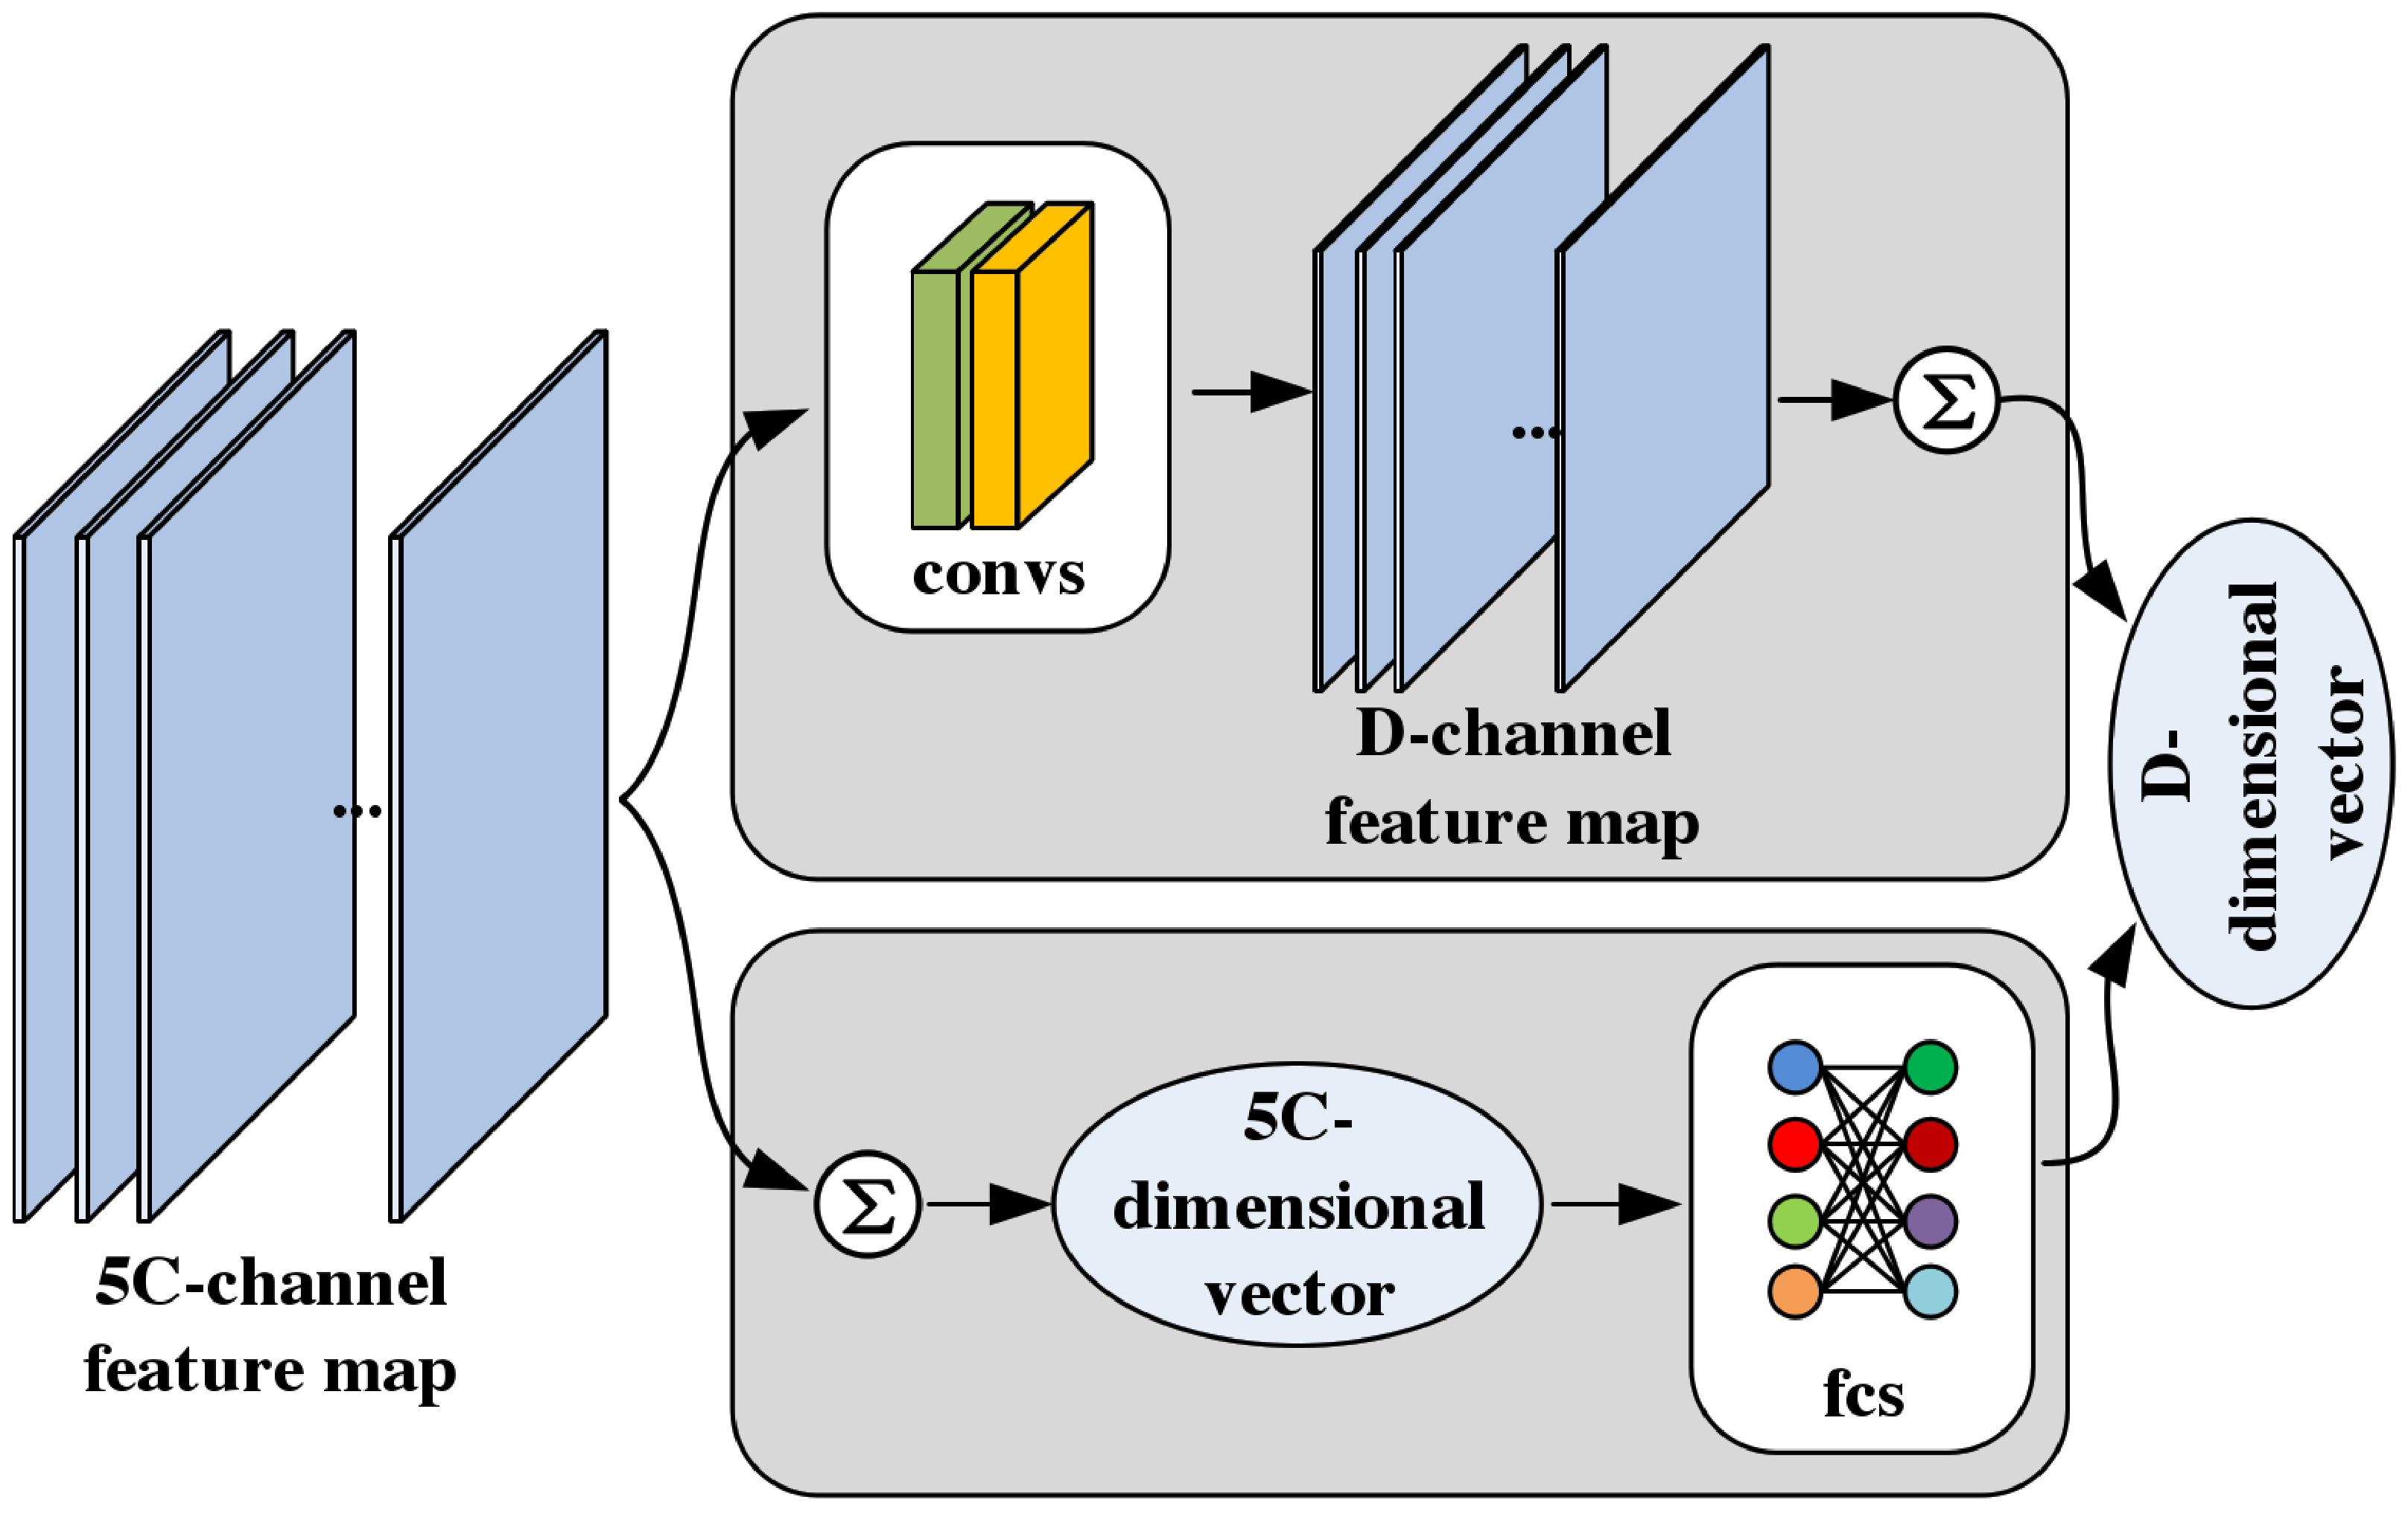
\includegraphics[width=65.02mm,height=40.64mm]{./zengyu_images/image009.eps}
\end{center}
Figure 4. Two different structures of the region embedding. The $\Sigma$ symbol denotes averaging over pixels of the region. Top and bottom streams indicates Conv-based and FC-based region em- beddin $\mathrm{g}$ respectively.

to get a $N^{2}\times C$-channel tensor of the input size. Then, the elements of the $N^{2}\times C$-channel tensor are rearranged into a $C$-channel output tensor of $N$ times the size of the input tensor.

Five $C$-channel feature maps can be produced though adding a subpixel convolution layer after each of the five convolution blocks. Then the five $C$-channel feature maps are cascaded into a $5C$-channel feature map. Directly us- ing the features of this $5C$-channel feature map to represent each pixel is not the best option since features of different convolution blocks are in different ranges. To solve this, we add two extra convolution layers after the subpixel convo- lution layers, to convert the $5C$-channel feature maps into a $D$-channel feature map, in which each pixel corresponds to a $D$-dimensional vector. In our implementation, we set $C$ to 64 and $D$ to 512.

3.4. Region embedding

$\mathrm{F}$or simplic ity, we let the pixel emb edding $\phi \theta$) and the the reg ion embeddin $\mathrm{g}\psi \eta$) sh are the common feature extractor and subpixel convolution upsample layers. New layers are append after the subpixel convolution layers to map the $5C$-channel feature map of an image region to a $D$-dimensional vector.

As shown in Figure 4, we consider two different struc- ture of the region embedding: Conv-based and FC-based re- gion embedding. In the Conv-based region embedding, the $5C$-channel feature map of an image region is passed into convolution layers, resulting in a $D$-channel feature map. Then the $D$-dimensional embedding vector is given by av- eraging the $D$-channel feature map over pixels. The FC- based region embedding uses fully connected layers to map the average over pixels of the $5C$-channel feature map into a $D$-dimensional vector.

4. Experiments 4.1. Datasets

We apply our method to five benchmark datasets to eval- uate its performance. Details of these datasets are as fol-

lows.

ECSSD $|31|$ contains 1000 natural images with multiple objects of different sizes. Some of the images come from the challenging Berkeley-300 dataset.

PASCAL-S $|19|$ stems from the validation set of PAS- CAL VOC2010 $|8|$ segmentation challenge and contains 850 natural images.

HKU-IS $|16|$ has 4447 images with high-quality pixel- wise annotations. Images in this dataset are chosen to in- clude multiple disconnected objects or objects touching the image boundary.

SOD $|31|$ has 300 images, and was originally designed for image segmentation. Pixel-wise annotations of salient objects were generated by $|13|$. This dataset is challenging since many images contain multiple objects either with low contrast or touching the image boundary.

DUTS $|27|$ is a large scale dataset containing 10533 training images and 5019 test images. All the training images are collected from the ImageNet DET training$/\mathrm{v}\mathrm{a}\mathrm{l}$ sets $|7|$, while test images are collected from the ImageNet DET test set and the SUN dataset $|30|$. Accurate pixel-level ground truths are provided.

4.2. Evaluation metrics

We employ Precision-Recall curve, $\mathrm{F}$-measure curve, F- measure score and MAE score to quantitatively evaluate the performance of the proposed method and compare with other methods.

The precision of a binary map is defined as the ratio of the number of salient pixels it correctly labels, to all salient pixels in this binary map. The recall value is the ratio of the number of correctly labeled salient pixels to all salient pixels in the ground-truth map:

precision $=\displaystyle \frac{|TS\cap DS|}{|DS|}$, recall $=\displaystyle \frac{|TS\cap DS|}{|TS|}$, (6)

in which $TS$ denotes true salient pixels, $DS$ denotes de- tected salient $\mathrm{p}$ ixels by the binary map, and $| |$ denotes cardinality of a set.

The F- measure, $\mathrm{d}$eno ted as $F_{\beta}$, is an overall $\mathrm{p}$ erformance indicator computed by the weighted harmonic of precision and recall:
\begin{center}
$F_{\beta}=\displaystyle \frac{(1+\beta^{2})\cdot \mathrm{p}\mathrm{r}\mathrm{e}\mathrm{c}\mathrm{i}\mathrm{s}\mathrm{i}\mathrm{o}\mathrm{n}\cdot \mathrm{r}\mathrm{e}\mathrm{c}\mathrm{a}\mathrm{l}1}{\beta^{2}\cdot \mathrm{p}\mathrm{r}\mathrm{e}\mathrm{c}\mathrm{i}\mathrm{s}\mathrm{i}\mathrm{o}\mathrm{n}+\mathrm{r}\mathrm{e}\mathrm{c}\mathrm{a}11}$,   (7)
\end{center}
where $\beta^{2}$ is set to 0.3 as suggested in $|1|$ to emphasize the precision.

Given a saliency map whose intensities are in the range of $0$ and 1, a series of binary maps can be produced by thresholding the saliency map with different values in $[0,$ 1]. Precision and recall values of these binary maps can be computed according to Eqn. $6_{\ovalbox{\tt\small REJECT}} \mathrm{F}$-measure can be computed

according to Eqn. 7. Plotting the (precision, recall) pairs of all the binary maps results in the precision-recall curve, and plotting the ($\mathrm{F}$-measure, threshold) pairs results in the $\mathrm{F}$-measure curve.

Also as suggested in $|1|$, we use twice the mean value of the saliency maps as the threshold to generate binary maps for computing the $\mathrm{F}$-measure. Notice that some works have reported slightly different $\mathrm{F}$-measures using different thresholds. But as far as we know, twice the mean value is the most commonly used threshold.

As complementary to PR curves, mean absolute error (MAE) is used to quantitatively measure the average dif- ference between the saliency map $S$ and the ground truth map $G$:

MAE $=\displaystyle \frac{1}{H}\sum_{i=1}^{H}|S_{i}-G_{i}|.$

MAE indicates how similar a saliency map is compared to the ground truth. It is widely used in different pixel-level prediction tasks such as semantic segmentation and image cropping [22].

4.3. Implementation details

Our method is implemented in Python with the PyTorch 1 toolbox. We train and test our model on a PC with a 3. $6\mathrm{G}\mathrm{H}\mathrm{z}$ CPU, $32\mathrm{G}\mathrm{B}$ RAM and a GTX 1080 GPU.

We train our model on the training set of DUTS dataset. As in $|20|$, we augment the training data by horizontal flip- ping and cropping the images to reduce overfitting. The probability $p$ of randomly flipping ground truth when pro- ducing anchors during training is set to 0.05. We compare two type of region embedding in Sec.4.4 , and adopt the Conv-based one in other experiments. Adam $|14|$ optimiza- tion method is used for training our model. Learning rate is set to le-3. We do not use a validation set, and train our model until its training loss converges. The training pro- cess takes almost 16 hours and converges after around $300\mathrm{k}$ iterations with mini-batch of size 1.

When comparing performance with other methods, the number of iterations $T$ in the iterative testing scheme (Alg. 2) is set to 1. We discuss the effect of larger $T$ val- ues in Sec.4.4 . When testing, the proposed method runs at about 15 fps with 256256 resolution on our computer with a 3. $6\mathrm{G}\mathrm{H}\mathrm{z}$ CPU and a GTX 1080 GPU. We release our code for future comparisons2 $\ovalbox{\tt\small REJECT}$

4.4. Ablation studies

Quantitative comparison between the two types of re- gion embedding is shown in Table 1. From this comparison

1https: $//$github. com/pytorch

2http: $//\mathrm{i}\mathrm{c}\mathrm{e}$. dlut. edu. $\mathrm{c}\mathrm{n}/\mathrm{l}\mathrm{u}/$

3https: $//$github. com/zengxianyu/lps
\begin{center}
\begin{tabular}{|l|l|l|l|}
\hline
\multicolumn{1}{|l|}{Baseline}&	\multicolumn{1}{|l|}{UCF}&	\multicolumn{1}{|l|}{RFCN}&	\multicolumn{1}{|l|}{ELD}	\\
\hline
\end{tabular}


\begin{tabular}{|l|l|l|l|l|l|l|}
\hline
\multicolumn{1}{|l|}{Methods}&	\multicolumn{1}{|l|}{$F_{\beta}$}&	\multicolumn{1}{|l|}{MAE}&	\multicolumn{1}{|l|}{$F_{\beta}$}&	\multicolumn{1}{|l|}{MAE}&	\multicolumn{1}{|l|}{$F_{\beta}$}&	\multicolumn{1}{|l|}{MAE}	\\
\hline
\multicolumn{1}{|l|}{BS}&	\multicolumn{1}{|l|}{$0.8394$}&	\multicolumn{1}{|l|}{ $0.0776$}&	\multicolumn{1}{|l|}{ $0.8337$}&	\multicolumn{1}{|l|}{ $0.1069$}&	\multicolumn{1}{|l|}{ $0.8098$}&	\multicolumn{1}{|l|}{ $0.0789$}	\\
\hline
\multicolumn{1}{|l|}{FC}&	\multicolumn{1}{|l|}{}&	\multicolumn{1}{|l|}{}&	\multicolumn{1}{|l|}{}&	\multicolumn{1}{|l|}{}&	\multicolumn{1}{|l|}{}&	\multicolumn{1}{|l|}{}	\\
\hline
\multicolumn{1}{|l|}{Conv}&	\multicolumn{1}{|l|}{}&	\multicolumn{1}{|l|}{}&	\multicolumn{1}{|l|}{}&	\multicolumn{1}{|l|}{}&	\multicolumn{1}{|l|}{}&	\multicolumn{1}{|l|}{}	\\
\hline
\end{tabular}

\end{center}
Table 1. Comparison in terms of $\mathrm{F}$-measure (the larger the better) and MAE (the smaller the better) between two types of region em- bedding evaluated on ECSSD dataset. The best and the second best methods are in red and green respectively. BS: baseline; FC: baseline promoted by the proposed method with FC-based region embedding; Conv: baseline promoted by the proposed method with Conv-based region embedding.
\begin{center}
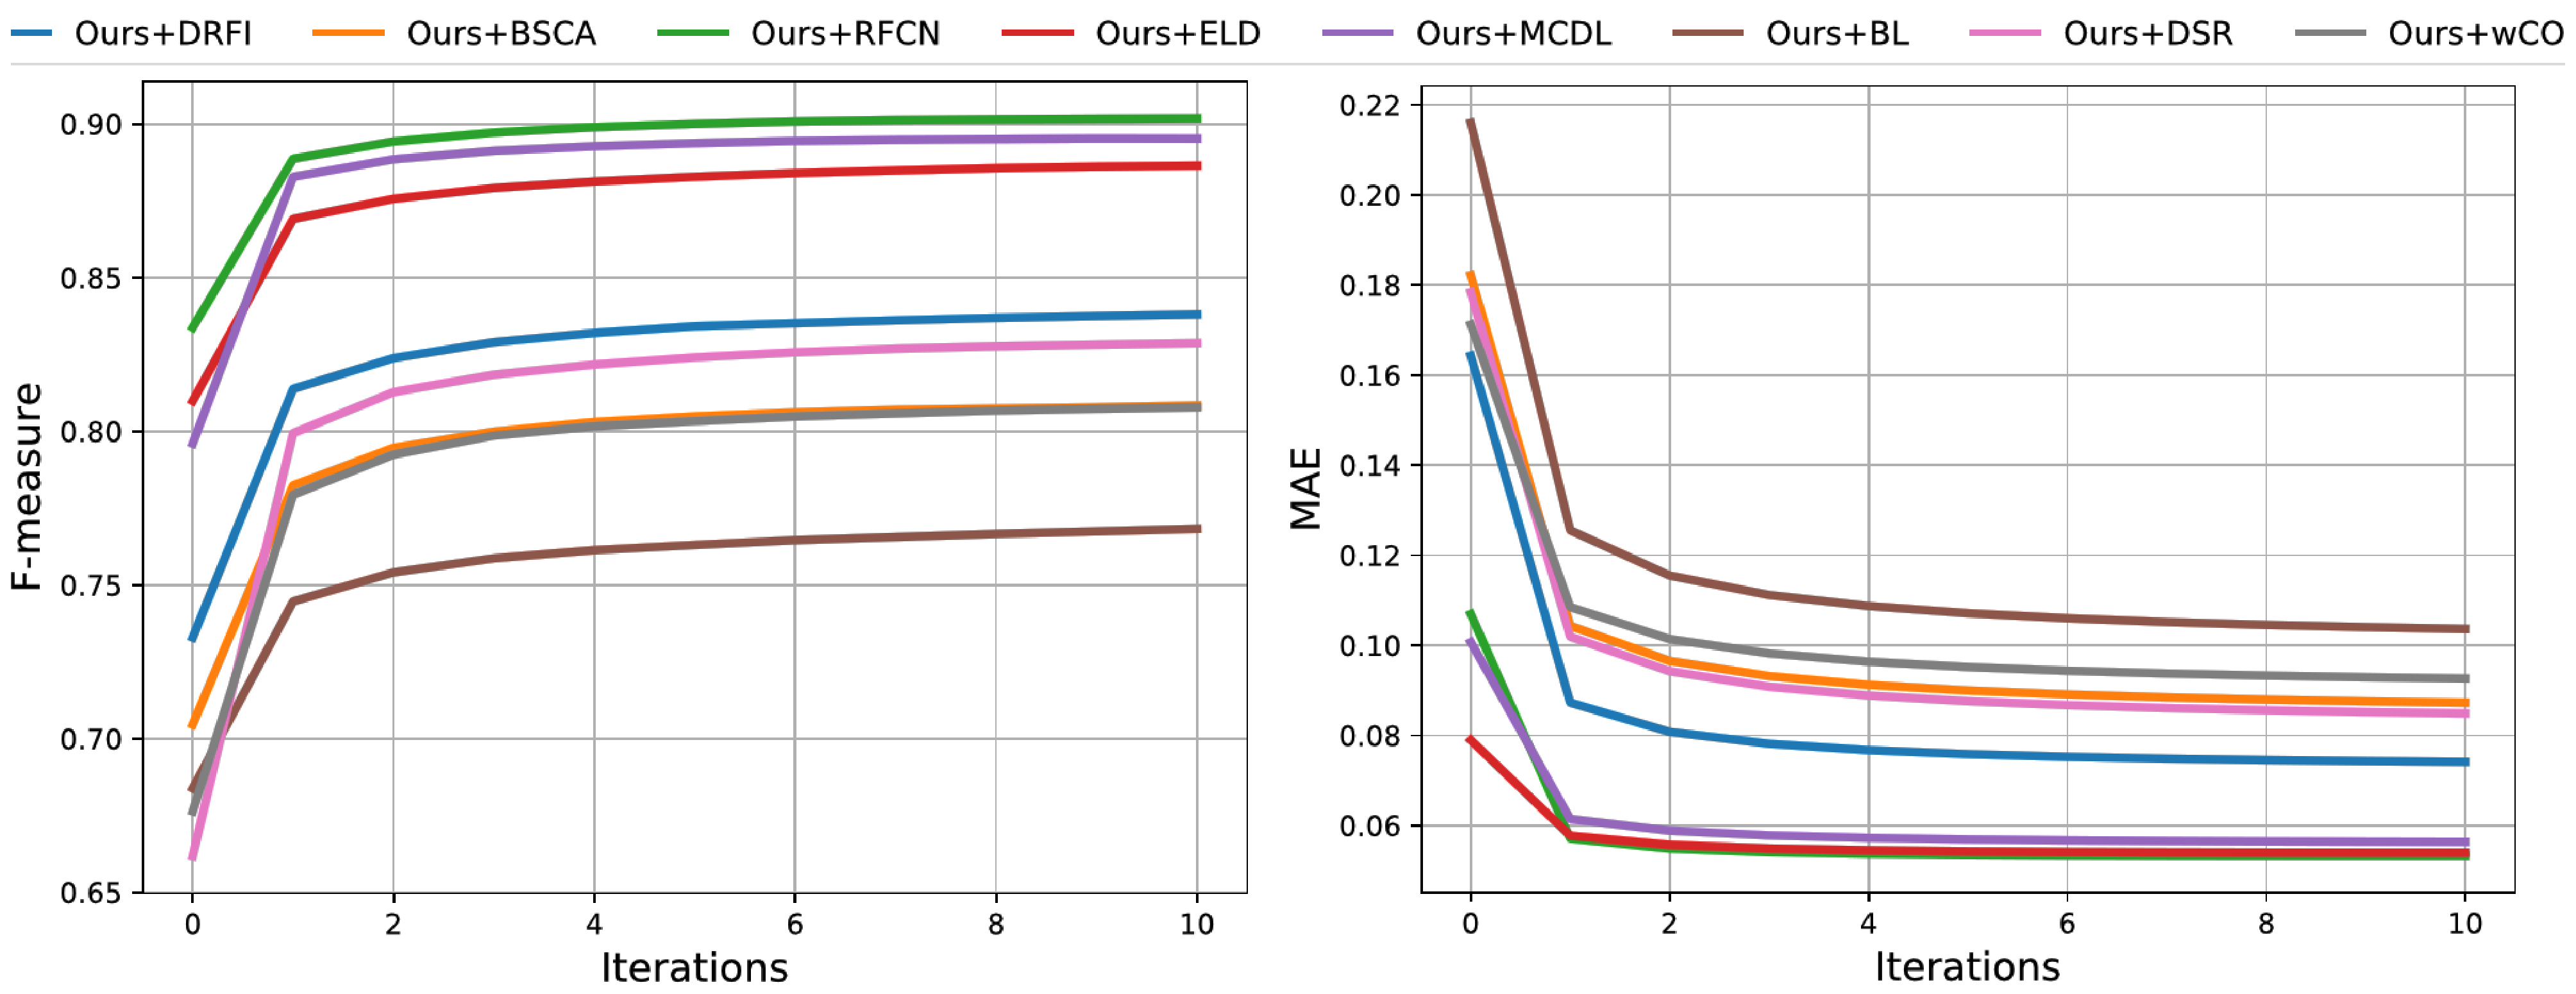
\includegraphics[width=80.94mm,height=30.82mm]{./zengyu_images/image010.eps}
\end{center}
Figure 5. Quantitative effect evaluated on ECSSD dataset in terms of $\mathrm{F}$-measure and MAE of the proposed iterative testing scheme. Different lines represents the effect of applying the proposed method on different algorithms.

we can see that the performance of FC-based and Conv- based region embedding is comparable. The FC-based re- gion embedding yields relatively larger $\mathrm{F}$-measure, while Conv-based region embedding is more superior in terms of

MAE.

We show the effect of the proposed iterative approxima- tion scheme in Figure 5. As shown in Figure 5, the first iteration improve the $\mathrm{F}$-measure and decrease MAE most significantly. The improvement slows down with iterations, and saturates gradually.

4.5. Performance

We choose 13 state-of-the-art methods as baselines, including 8 deep learning based methods (Amulet [34],

SRM $|29|$, UCF $|35|$, DHS $|20|$, NLDF $|21|$, ELD [15], RFCN $|28|$, DSS $|11$ and 5 conventional contenders

(BSCA $|23|$, DRFI $|13|, \mathrm{w}\mathrm{C}\mathrm{O}|36|$, DSR $|17|$, BL [26]). We apply our method to promote the performance of each baseline method, by using its predicted saliency maps to generate initial anchors in Eqn.3. Figure 6 shows the PR curves of the baseline methods and the one promoted by our method. Table 2 shows the $\mathrm{F}$-measure and MAE scores of 8 deep learning based methods and the corresponding pro- moted results. The quantified improvements in $\mathrm{F}$-measure and MAE of applying our method to conventional methods are shown in Table 3. As shown in Figure 6, Table 2, and Table 3, our method drastically promotes all the baseline methods.

Based on our results, we make several fundamental ob-

AmuIet ELD DSS DRFI $\mathrm{O}\mathrm{u}\mathrm{r}\mathrm{s}+$AmuIet $\mathrm{O}\mathfrak{u}\mathrm{r}\mathrm{s}+\mathrm{E}\mathrm{L}\mathrm{D} \mathrm{O}\mathrm{u}r\mathrm{s}+\mathrm{D}\mathrm{S}\mathrm{S} \mathrm{O}\mathrm{u}\mathrm{r}\mathrm{s}+$DRFl DHS RFCN BSCA wCO Ou $\mathrm{r}\mathrm{s}+\mathrm{D}\mathrm{H}\mathrm{S} \mathrm{O}\mathfrak{u}\mathrm{r}\mathrm{s}+$RFCN Ours$+$BSCA -- $\mathrm{O}\mathrm{u}\mathrm{r}\mathrm{s}+\mathrm{w}\mathrm{C}\mathrm{O}$
\begin{center}
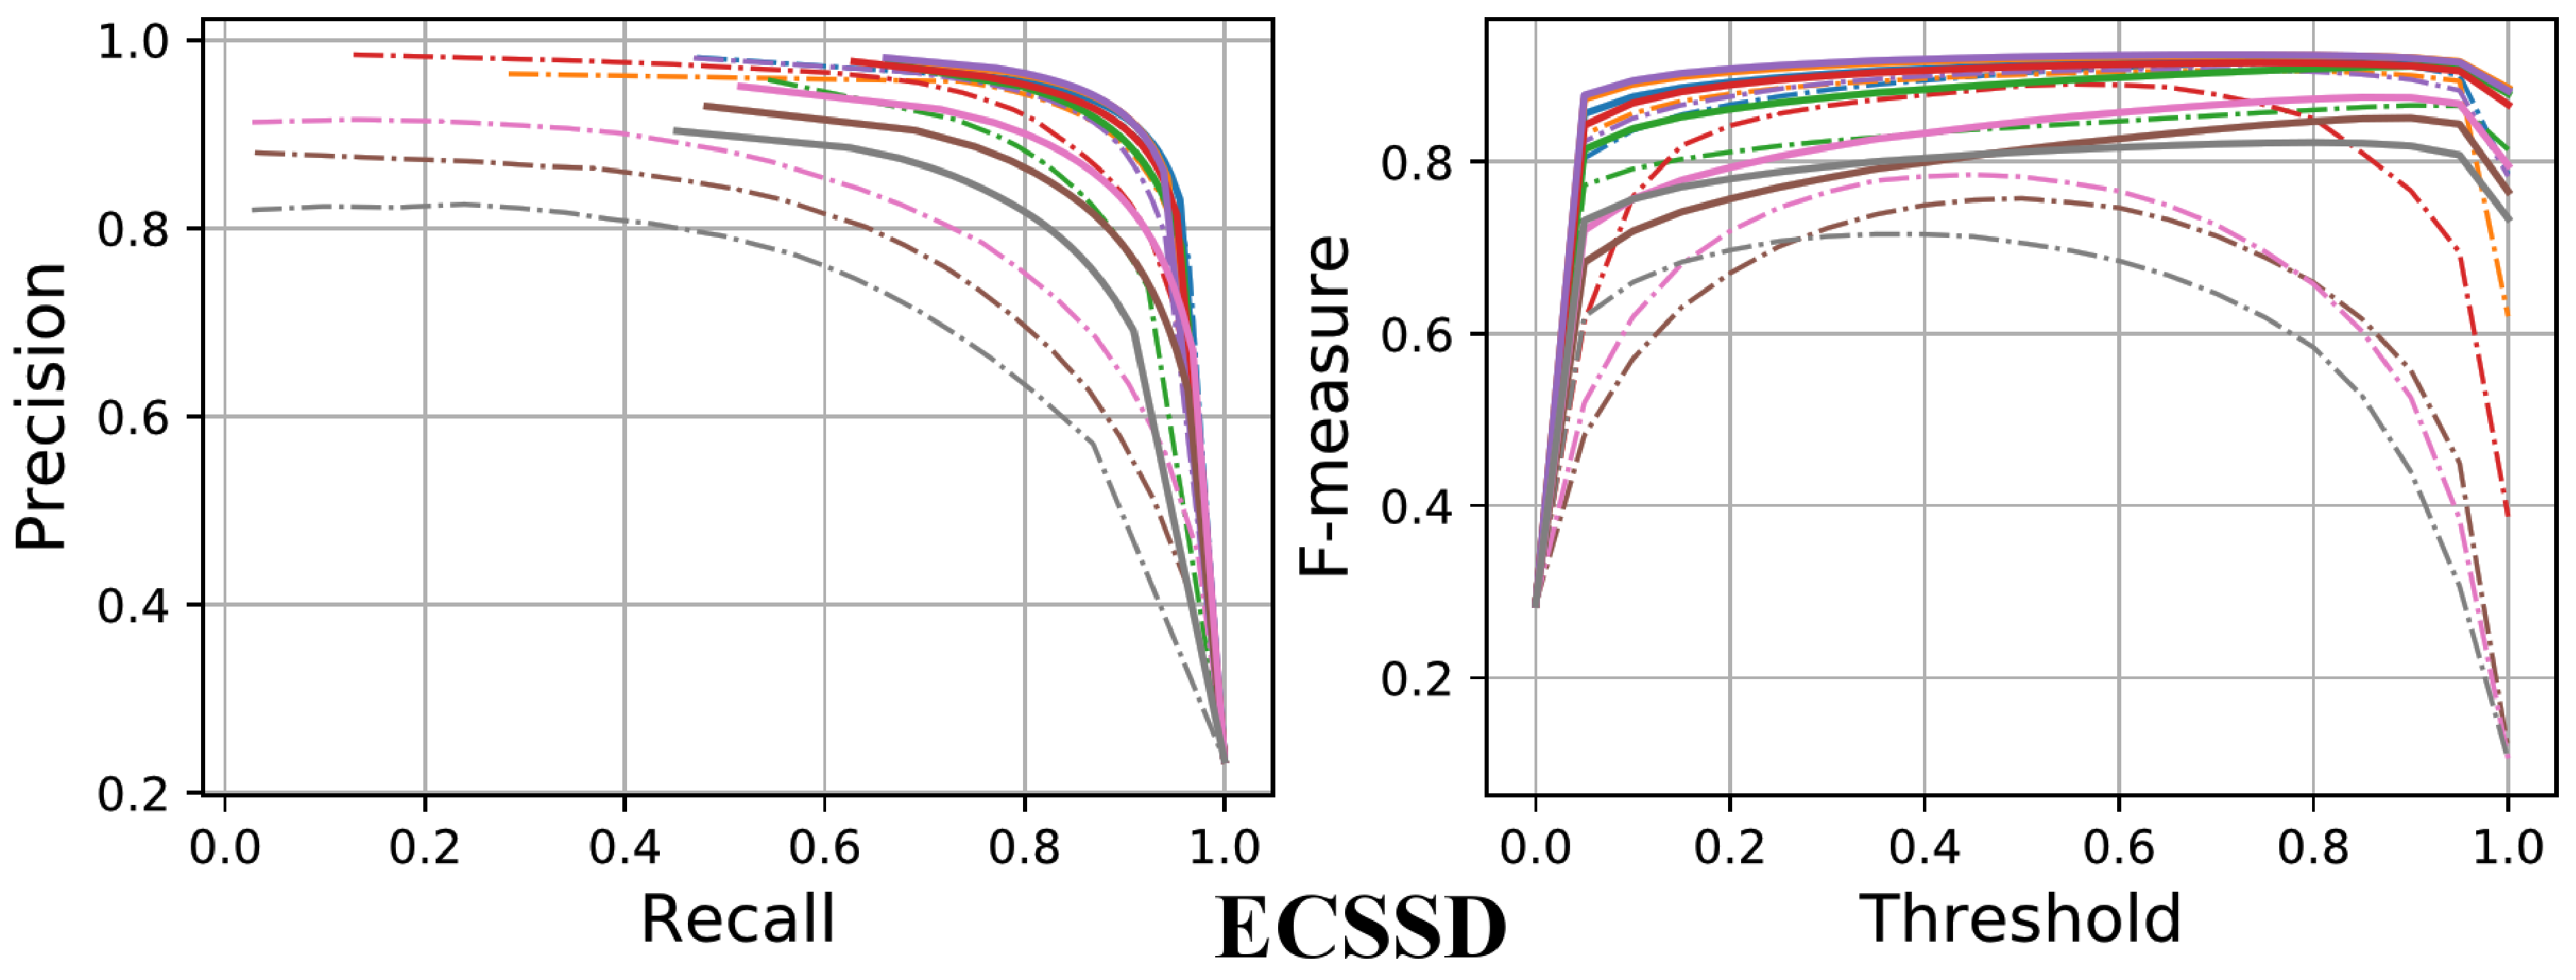
\includegraphics[width=75.86mm,height=28.45mm]{./zengyu_images/image011.eps}

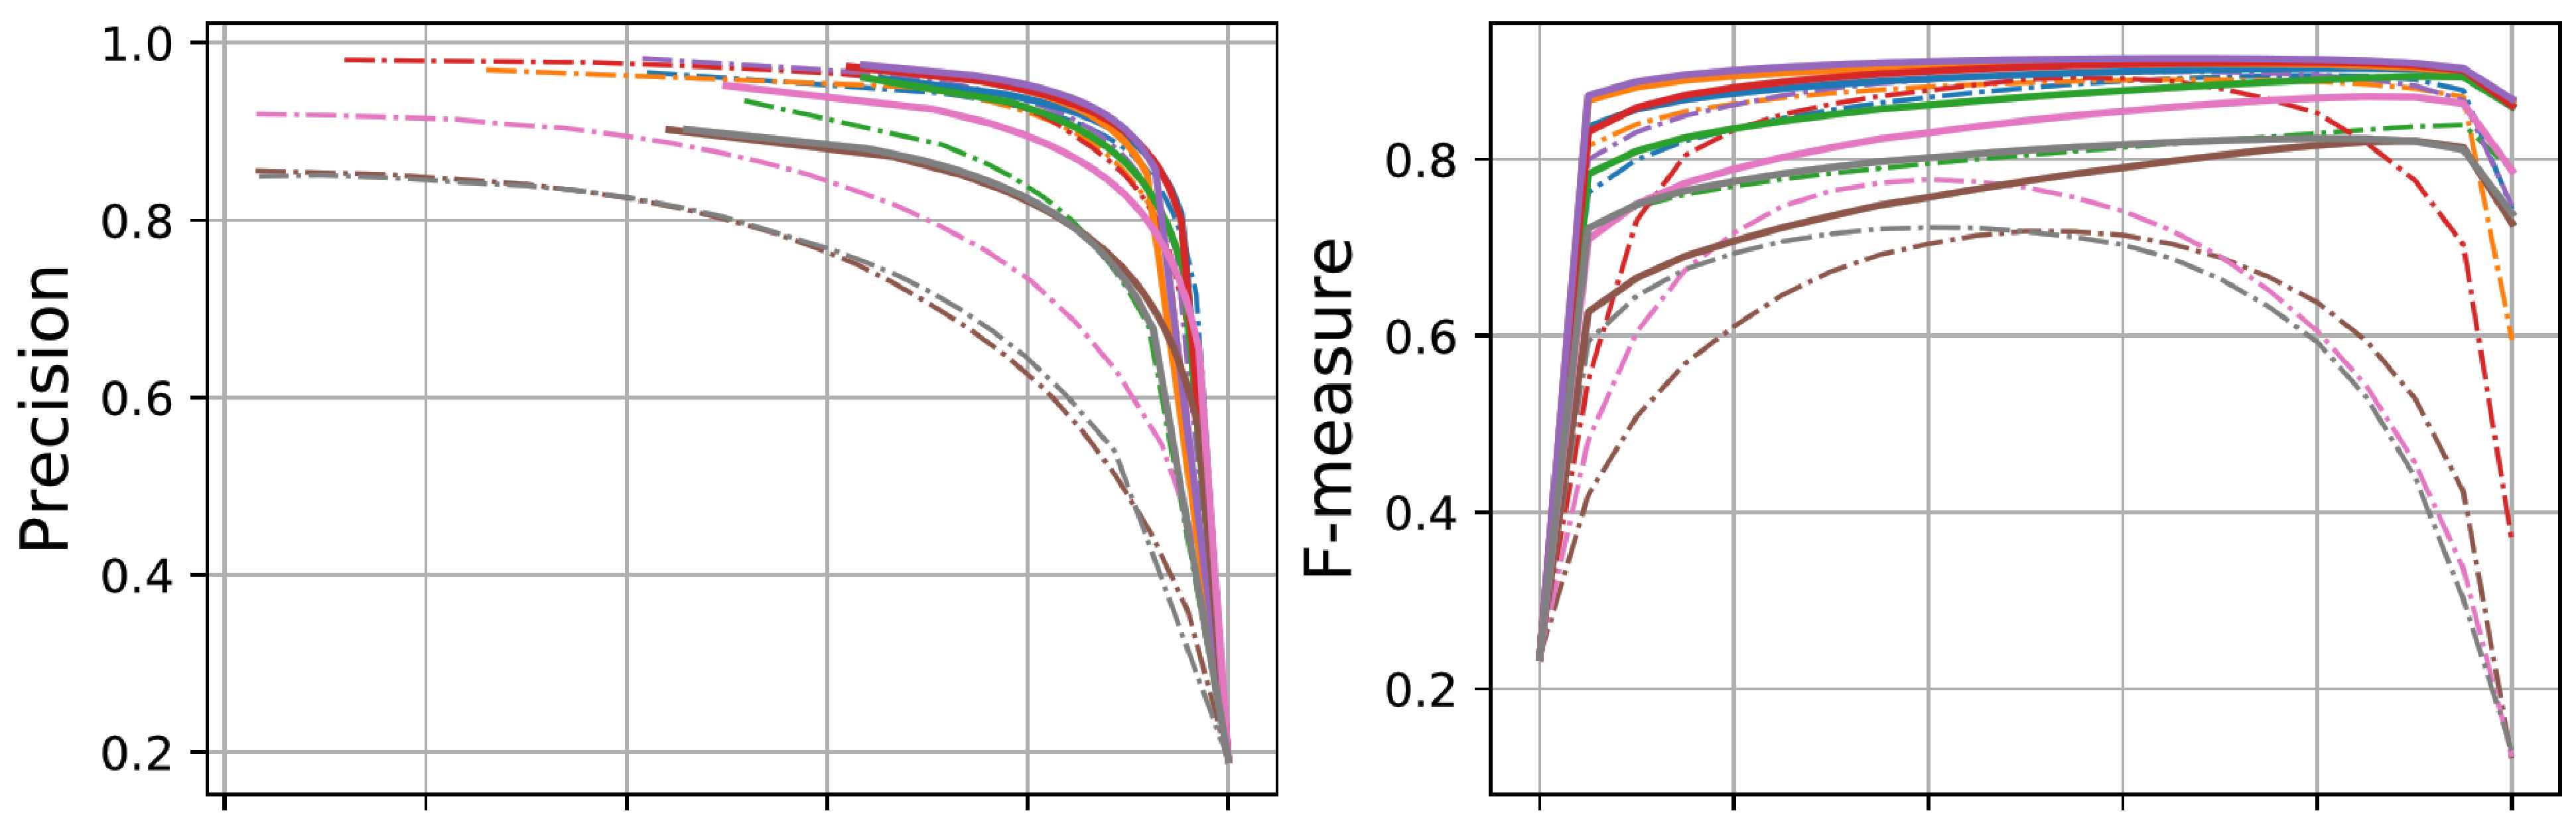
\includegraphics[width=78.23mm,height=24.51mm]{./zengyu_images/image012.eps}
$$
0\ 0\ 0\ 0\ 0\ 1\ 0\ 0\ 0\ 0\ 0\ 1
$$
\end{center}
Recall Th $\ulcorner$eshold

HKU-IS
\begin{center}
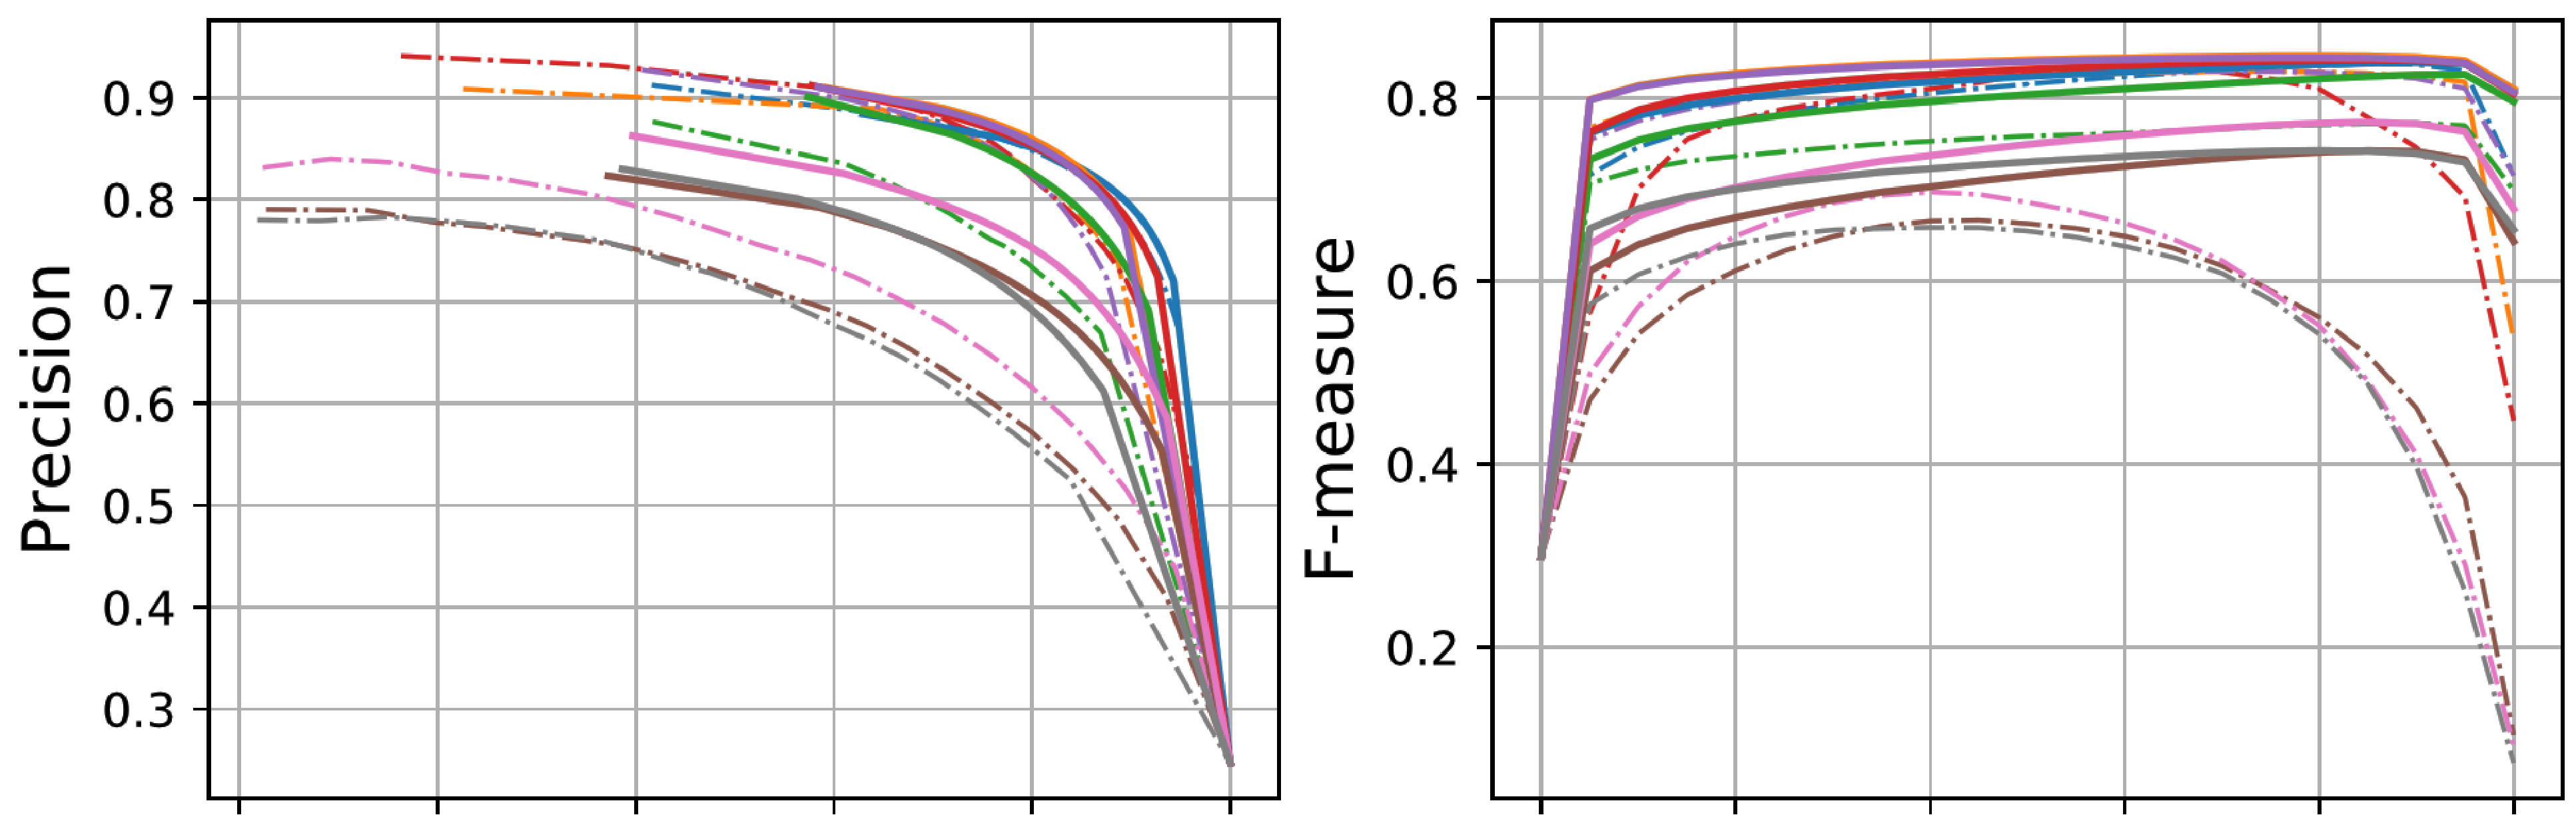
\includegraphics[width=77.89mm,height=24.55mm]{./zengyu_images/image013.eps}
$$
0\ 0\ 0\ 0\ 0\ 1\ 0\ 0\ 0\ 0\ 0\ 1
$$
\end{center}
Recall Th reshold

PASCAL-S
\begin{center}
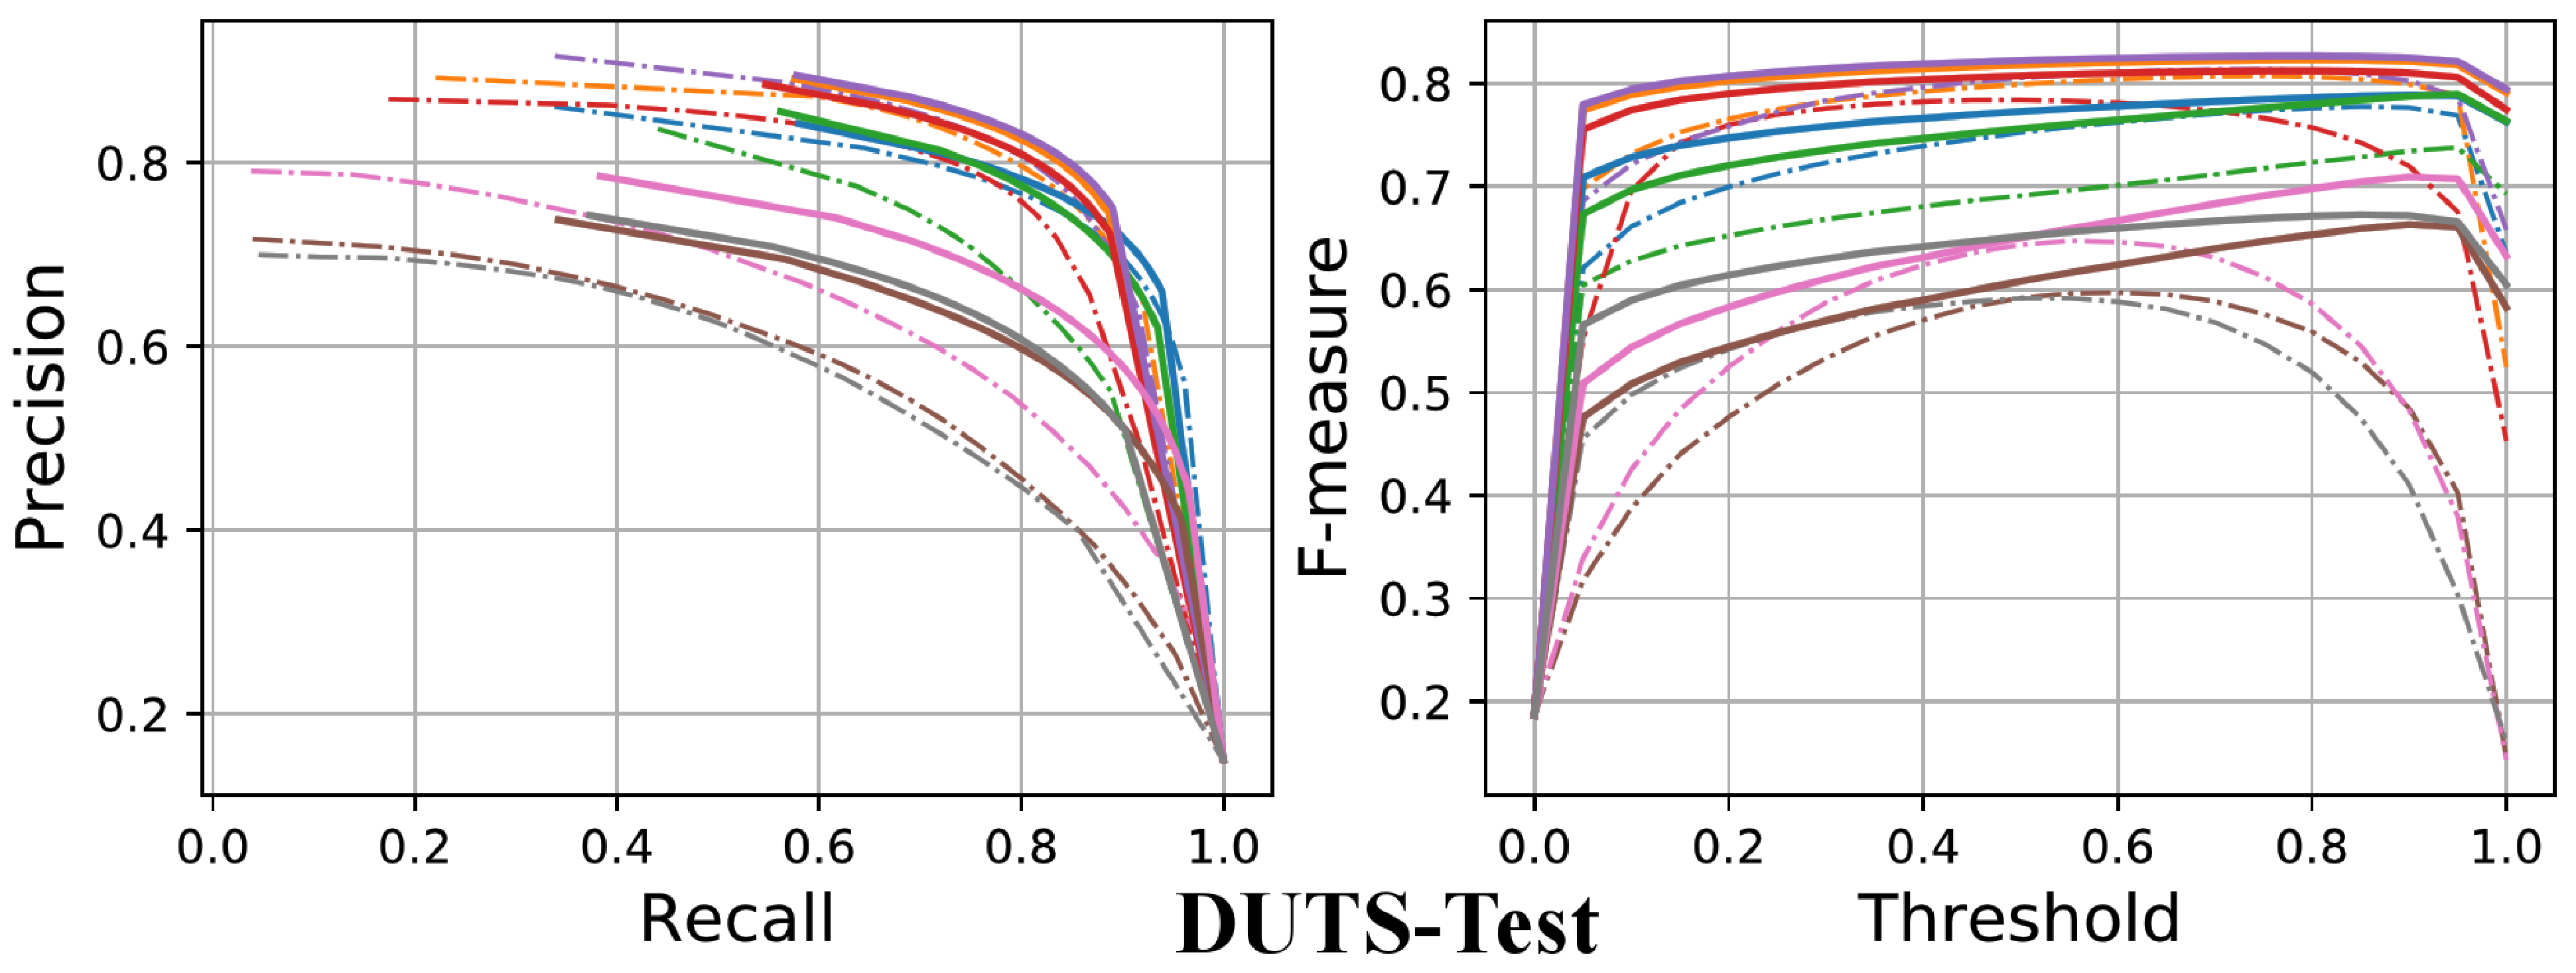
\includegraphics[width=78.23mm,height=29.13mm]{./zengyu_images/image014.eps}

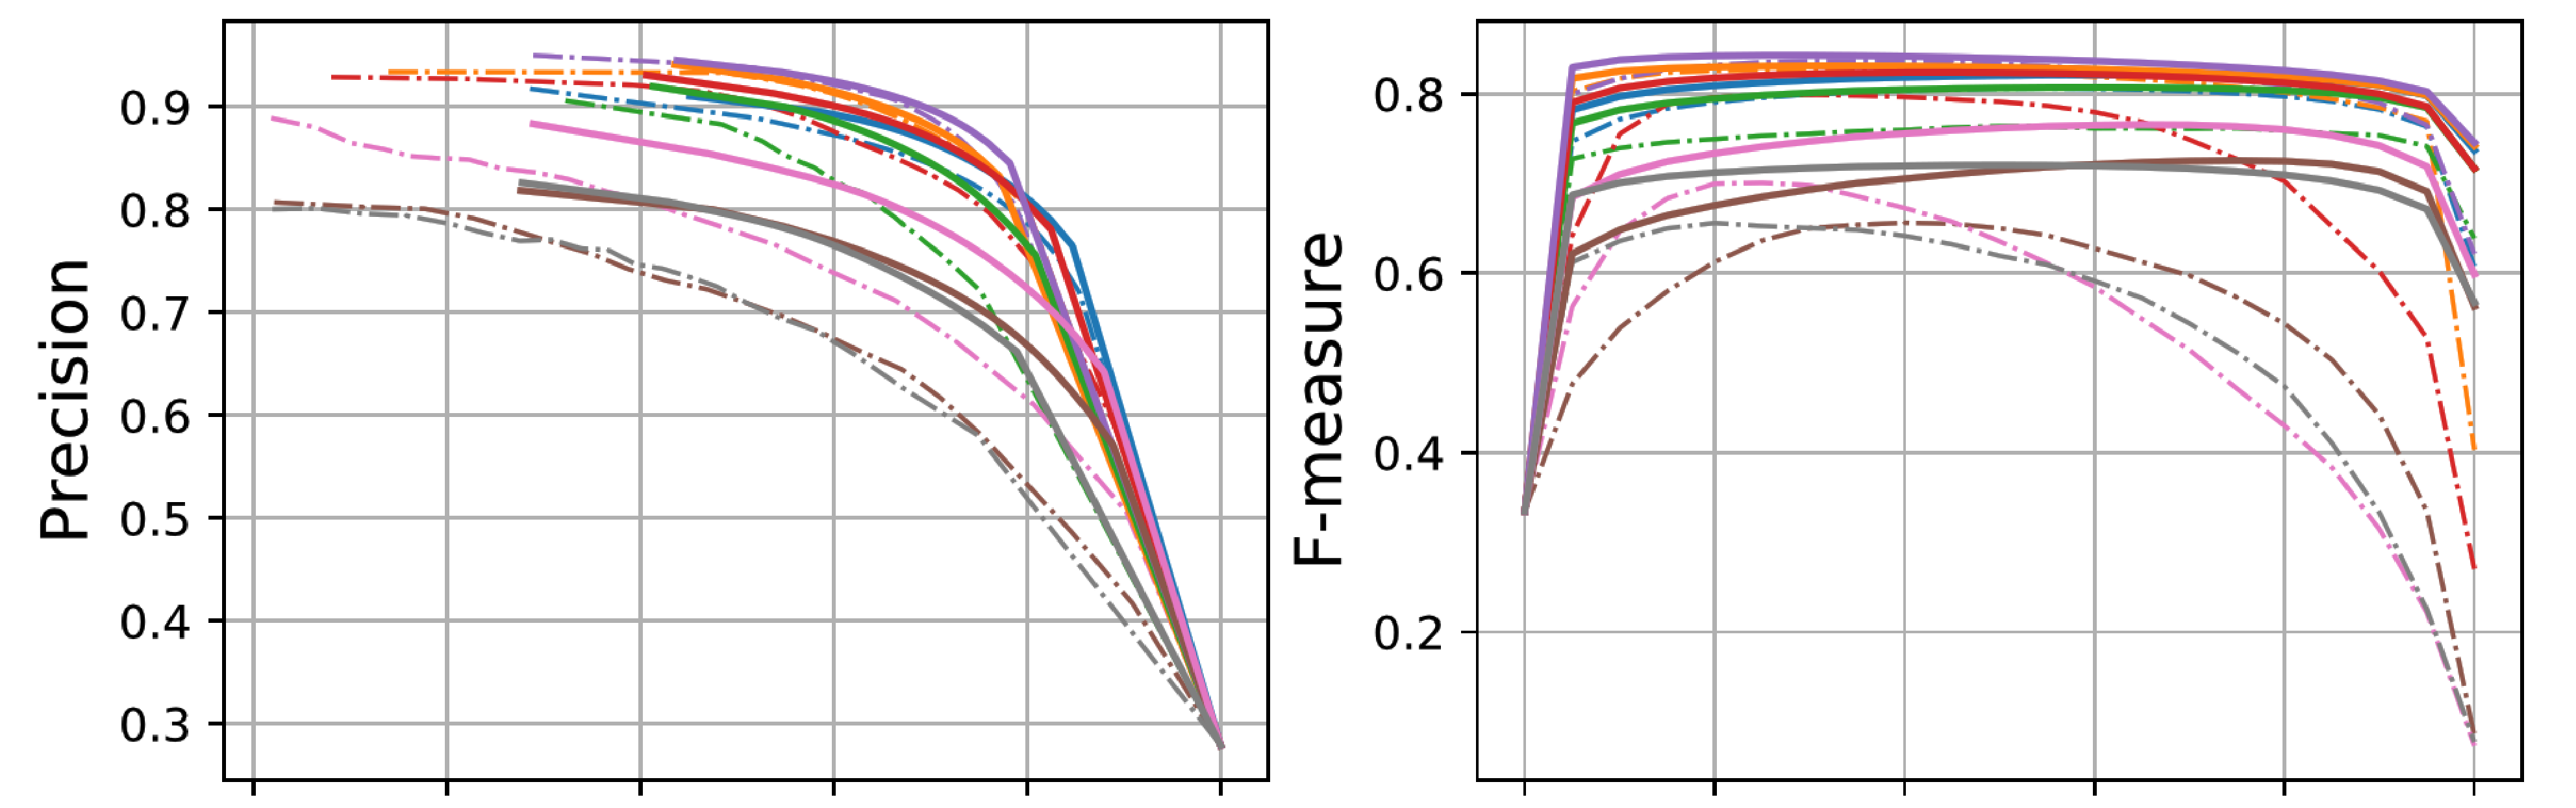
\includegraphics[width=79.93mm,height=24.60mm]{./zengyu_images/image015.eps}
\end{center}
$0$
$$
0
$$
$$
0
$$
$$
0
$$
$$
0
$$
1
$$
0
$$
$$
0
$$
$$
0
$$
$$
0
$$
$$
0
$$
1

Recall SOD Threshold

Figure 6. PR curves and $\mathrm{F}$-measure curves of our method and the the state-of-the-art methods.

servations:

1. Our proposed method decreases the MAE of SRM, the best-performing method to date, by 15.3\% on HKU-IS dataset and 14.2\% on ECSSD dataset.

2. Although our method is based on deep learning, it also performs well when applied to conventional methods. For instance, our method decreases the MAE of DRFI by around 50\% on both ECSSD and HKU-IS datasets. Our method does not rely on any specific choice of the initial map, and generalizes well across different baseline methods.

ECSSD

HKU-IS

PASCALS

DUTS-Test

SOD
\begin{center}

\includegraphics[width=175.34mm,height=3.64mm]{./zengyu_images/image016.eps}
\end{center}
Methods

Amulet

SRM

UCF

DHS
\begin{center}
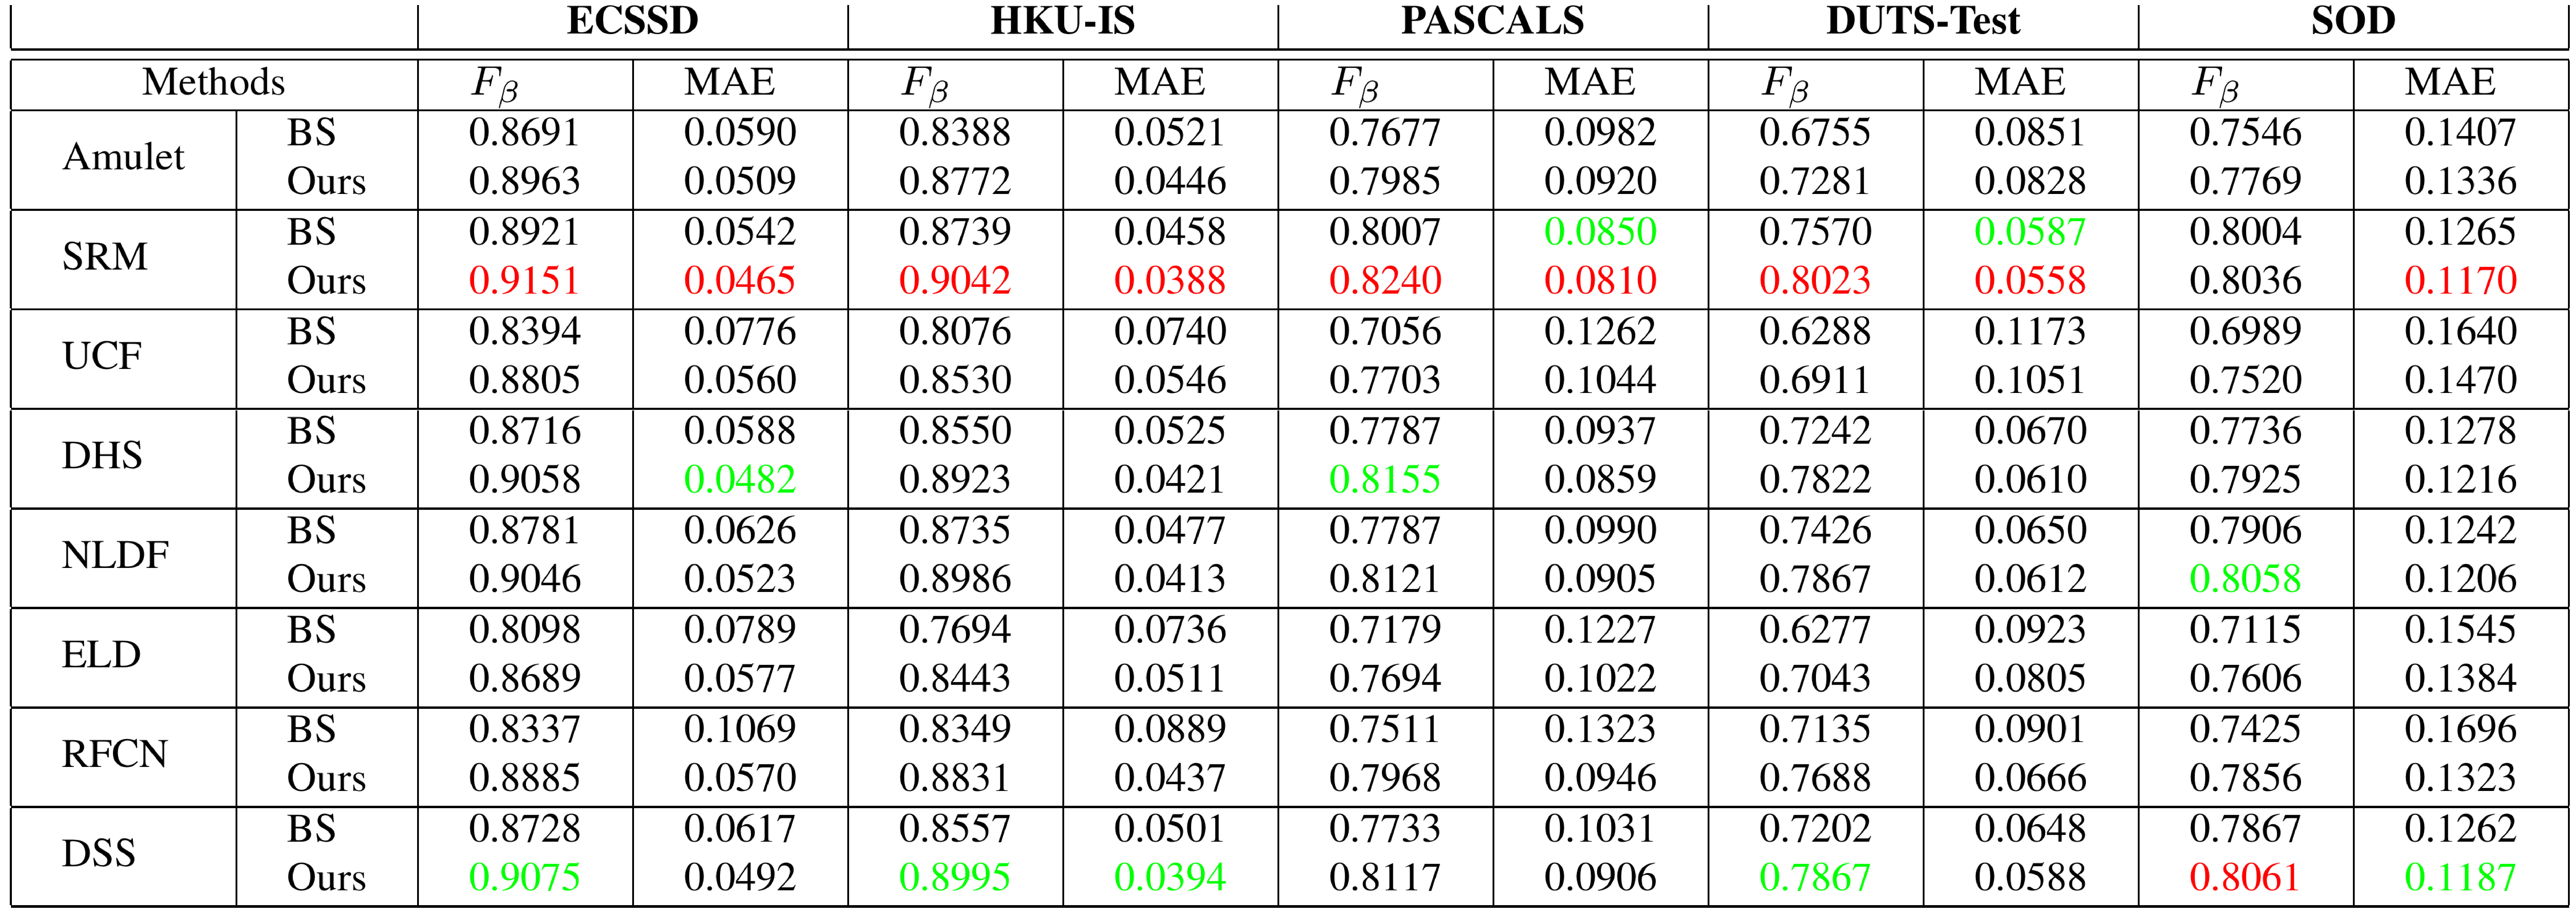
\includegraphics[width=175.77mm,height=62.15mm]{./zengyu_images/image017.eps}
\end{center}
NLDF

ELD

RFCN

DSS

BS Ours BS Ours BS Ours BS Ours BS Ours BS Ours BS Ours BS Ours

$\mathrm{F}_{\beta}$ 0.8691 0.8963 0.8921 0.9151 0.8394 0.8805 0.8716 0.9058 0.8781 0.9046 0.8098 0.8689 0.8337 0.8885 0.8728 0.9075

MAE 0.0590 0.0509 0.0542 0.0465 0.0776 0.0560 0.0588 0.0482 0.0626 0.0523 0.0789 0.0577 0.1069 0.0570 0.0617 0.0492

$\mathrm{F}_{\beta}$ 0.8388 0.8772 0.8739 0.9042 0.8076 0.8530 0.8550 0.8923 0.8735 0.8986 0.7694 0.8443 0.8349 0.8831 0.8557 0.8995

MAE 0.0521 0.0446 0.0458 0.0388 0.0740 0.0546 0.0525 0.0421 0.0477 0.0413 0.0736 0.0511 0.0889 0.0437 0.0501 0.0394

$\mathrm{F}_{\beta}$ 0.7677 0.7985 0.8007 0.8240 0.7056 0.7703 0.7787 0.8155 0.7787 0.8121 0.7179 0.7694 0.7511 0.7968 0.7733 0.8117

MAE 0.0982 0.0920 0.0850 0.0810 0.1262 0.1044 0.0937 0.0859 0.0990 0.0905 0.1227 0.1022 0.1323 0.0946 0.1031 0.0906

$\mathrm{F}_{\beta}$ 0.6755 0.7281 0.7570 0.8023 0.6288 0.6911 0.7242 0.7822 0.7426 0.7867 0.6277 0.7043 0.7135 0.7688 0.7202 0.7867

MAE 0.0851 0.0828 0.0587 0.0558 0.1173 0.1051 0.0670 0.0610 0.0650 0.0612 0.0923 0.0805 0.0901 0.0666 0.0648 0.0588

$\mathrm{F}_{\beta}$ 0.7546 0.7769 0.8004 0.8036 0.6989 0.7520 0.7736 0.7925 0.7906 0.8058 0.7115 0.7606 0.7425 0.7856 0.7867 0.8061

MAE 0.1407 0.1336 0.1265 0.1170 0.1640 0.1470 0.1278 0.1216 0.1242 0.1206 0.1545 0.1384 0.1696 0.1323 0.1262 0.1187

Table 2. Comparison in terms of $\mathrm{F}$-measure (the larger the better) and MAE (the smaller the better) score of our method against other deep learning based methods. The best and the second best methods are in red and green respectively. BS: the baseline; Ours: the promoted result of applying our method on the baseline.

ECSSD

HKU-IS

PASCALS

DUTS-Test

SOD
\begin{center}

\includegraphics[width=174.24mm,height=3.64mm]{./zengyu_images/image018.eps}
\end{center}
Methods

BSCA

DRFI
\begin{center}
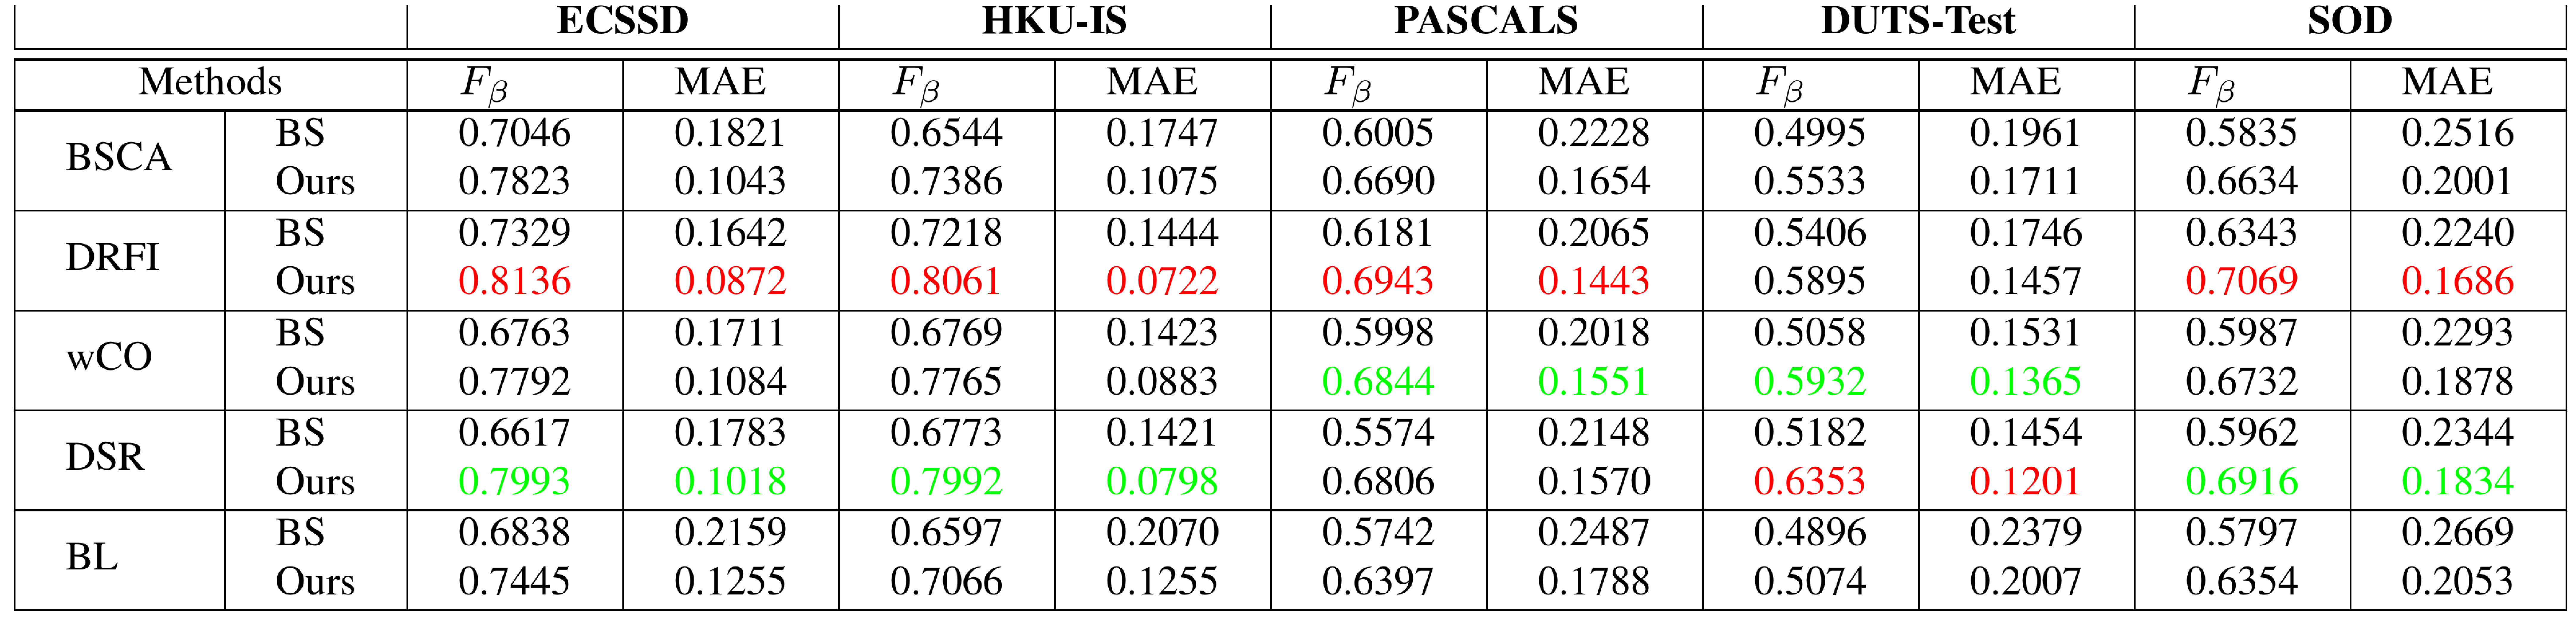
\includegraphics[width=175.09mm,height=41.49mm]{./zengyu_images/image019.eps}
\end{center}
$\mathrm{w}\mathrm{C}0$

DSR

BL

BS Ours BS Ours BS Ours BS Ours BS Ours

$\mathrm{F}_{\beta}$ 0.7046 0.7823 0.7329 0.8136 0.6763 0.7792 0.6617 0.7993 0.6838 0.7445

MAE 0.1821 0.1043 0.1642 0.0872 0.1711 0.1084 0.1783 0.1018 0.2159 0.1255

$\mathrm{F}_{\beta}$ 0.6544 0.7386 0.7218 0.8061 0.6769 0.7765 0.6773 0.7992 0.6597 0.7066

MAE 0.1747 0.1075 0.1444 0.0722 0.1423 0.0883 0.1421 0.0798 0.2070 0.1255

$\mathrm{F}_{\beta}$ 0.6005 0.6690 0.6181 0.6943 0.5998 0.6844 0.5574 0.6806 0.5742 0.6397

MAE 0.2228 0.1654 0.2065 0.1443 0.2018 0.1551 0.2148 0.1570 0.2487 0.1788

$\mathrm{F}_{\beta}$ 0.4995 0.5533 0.5406 0.5895 0.5058 0.5932 0.5182 0.6353 0.4896 0.5074

MAE 0.1961 0.1711 0.1746 0.1457 0.1531 0.1365 0.1454 0.1201 0.2379 0.2007

$\mathrm{F}_{\beta}$ 0.5835 0.6634 0.6343 0.7069 0.5987 0.6732 0.5962 0.6916 0.5797 0.6354

MAE 0.2516 0.2001 0.2240 0.1686 0.2293 0.1878 0.2344 0.1834 0.2669 0.2053

Table 3. Comparison in terms of $\mathrm{F}$-measure (the larger the better) and MAE (the smaller the better) score of our method against the conventional methods. The best and the second best methods are in red and green respectively. BS: the baseline; Ours: the promoted result of applying our method on the baseline.

3. Notice that the results shown here are obtained by iter- ating Alg. 2 only once for fast testing speed. As shown in Sec.4.4 , better results can be achieved through iter- ating Alg. 2 more times.
\begin{center}
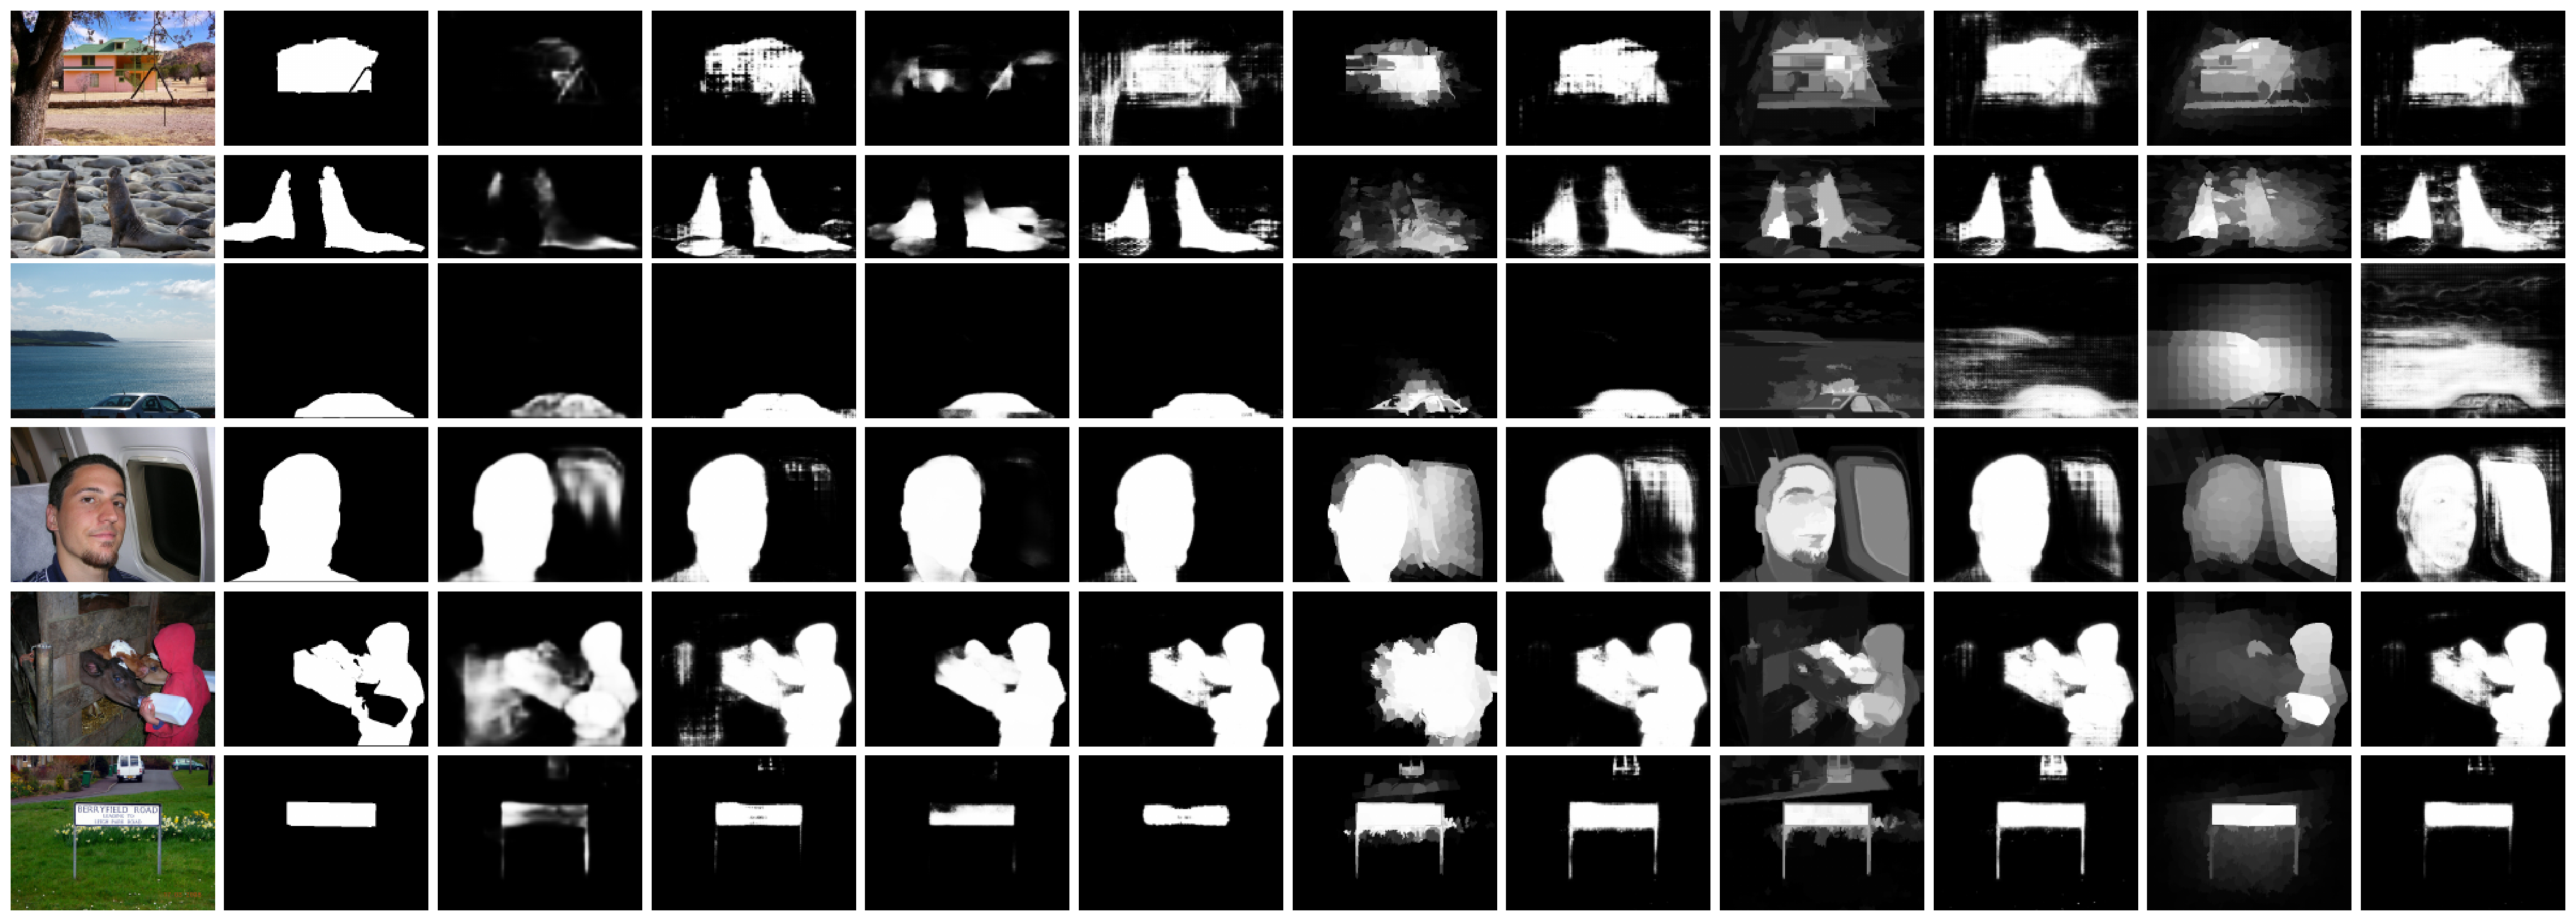
\includegraphics[width=83.02mm,height=29.25mm]{./zengyu_images/image020.eps}
\end{center}
Figure 7 shows a visual comparison of saliency maps pro- duced by some state-of-the-art methods and the promoted ones by our method. It can be seen that the saliency maps produced by our methods highlight salient regions that are missed by the baselines. Further, our method can suppress the background regions that are wrongly labeled as salient by the baseline methods.

Figure 7 shows a visual comparison of saliency maps pro- duced by some state-of-the-art methods and the promoted ones by our method. It can be seen that the saliency maps produced by our methods highlight salient regions that are missed by the baselines. Further, our method can suppress the background regions that are wrongly labeled as salient by the baseline methods.

Figure 7 shows a visual comparison of saliency maps pro- duced by some state-of-the-art methods and the promoted ones by our method. It can be seen that the saliency maps produced by our methods highlight salient regions that are missed by the baselines. Further, our method can suppress the background regions that are wrongly labeled as salient by the baseline methods.

input GT SRM $+\mathrm{S}\mathrm{R}\mathrm{M}$ NLDF $+$NLDF ELD $+\mathrm{E}\mathrm{L}\mathrm{D}$ DRFI $+$DRFI BSCA $+$BSCA Figure 7. Visual comparison of the algorithms promoted by our method against the baseline algorithms. Input: input images; GT: ground truth maps; A plus sign denotes the algorithm promoted by our method.

5. Conclusion

Acknowledgment

In this paper, we propose a novel learning method to promote existing salient object detection methods. Ex- tensive experiments on five benchmark datasets show that our method can significantly improve accuracy of existing methods and compares favorably against state-of-the-arts.

In this paper, we propose a novel learning method to promote existing salient object detection methods. Ex- tensive experiments on five benchmark datasets show that our method can significantly improve accuracy of existing methods and compares favorably against state-of-the-arts.

This work was supported by the Natural Science Foun- dation of China under Grant 61725202, 61472060 and 61371157. In addition, the authors would like to thank Li- jun Wang, Hongshuang Zhang and Yunhua Zhang for their help.

References

[1] R. Achanta, S. Hemami, F. Estrada, and S. Susstrunk. Frequency-tuned salient region detection. In {\it Computer vi}- {\it sion and pattern recognition, 2009. cvpr 2009. ieee confer}- {\it ence on}, pages 1597-1604. IEEE, 2009.

[2] R. Achanta and S. S"\""{u}"sstrunk. Saliency detection for content- aware image resizing. In {\it Image Processing} ({\it ICIP}), {\it 2009 16th IEEE International Conference on}, pages 1005-1008. IEEE, 2009.

[3] A. Borji. Boosting bottom-up and top-down visual features for saliency estimation. In {\it Proceedings of the IEEE Con}- {\it ference on Computer Vision and Pattern Recognition}, pages

438 445. IEEE, 2012.

[4] A. Borji, M.-M. Cheng, H. Jiang, and J. Li. Salient object detection: A benchmark. {\it IEEE Transactions on Image Pro}- {\it cessing}, $24(12):5706-5722$, 2015.

[5] A. Borji and L. Itti. State-of-the-art in visual attention mod- eling. {\it IEEE transactions on pattern analysis and machine intelligence}, 35(1): 185 207, 2013.

[6] A. Borji, D. N. Sihite, and L. Itti. Quantitative analysis of human-model agreement in visual saliency modeling: $\mathrm{A}$ comparative study. {\it IEEE Transactions on Image Processing},
\begin{center}
$22(1):55-69$, 2013.
\end{center}
[7] J. Deng, W. Dong, R. Socher, L.-J. Li, K. Li, and L. Fei- Fei. Imagenet: A large-scale hierarchical image database. In {\it Proceedings of the IEEE Conference on Computer Vision and Pattern Recognition}, pages 248 255. IEEE, 2009.

[8] M. Everingham, L. Van Gool, C. K. Williams, J. Winn, and A. Zisserman. The pascal visual object classes (voc) chal- lenge. {\it International journal of computer vision}, $88(2):303-$
\begin{center}
338, 2010.
\end{center}
[9] D. Gao, S. Han, and N. Vasconcelos. Discriminant saliency, the detection of suspicious coincidences, and applications to visual recognition. {\it IEEE Transactions on Pattern Analysis and Machine Intelligence}, 31 (6):989-1005, 2009.

[10] Y. Gao, M. Wang, Z.-J. Zha, J. Shen, X. Li, and X. Wu. Visual-textual joint relevance learning for tag-based social image search. {\it IEEE Transactions on Image Processing},
\begin{center}
$22(1):363-376$, 2013.
\end{center}
[11] Q. Hou, M.-M. Cheng, X. Hu, A. Borji, Z. Tu, and P. Torr. Deeply supervised salient object detection with short connections. In {\it Computer Vision and Pattern Recogni}- {\it tion} ({\it CVPR}), {\it 2017 IEEE Conference on}, pages 5300 5309. IEEE, 2017.

[12] B. Jiang, L. Zhang, H. Lu, C. Yang, and M.-H. Yang. Saliency detection via absorbing markov chain. In {\it Proceed}- {\it ings of the IEEE International Conference on Computer Vi}- {\it sion}, pages 1665-1672, 2013.

[13] H. Jiang, J. Wang, Z. Yuan, Y. Wu, N. Zheng, and S. Li. Salient object detection: A discriminative regional feature integration approach. In {\it Proceedings of the IEEE conference on computer vision and pattern recognition}, pages 2083- 2090, 2013.

[14] D. Kingma and J. Ba. Adam: A method for stochastic opti- mization. {\it arXiv preprint arXiv}:{\it 1412.6980}, 2014.

[15] G. Lee, Y.-W. Tai, and J. Kim. Deep saliency with encoded low level distance map and high level features. In {\it Proceed}-

{\it ings of the IEEE Conference on Computer Vision and Pattern Recognition}, pages 660 668, 2016.

[16] G. Li and Y. Yu. Visual saliency based on multiscale deep features. In {\it Proceedings of the IEEE conference on computer vision and pattern recognition}, pages 5455 5463, 2015.

[17] X. Li, H. Lu, L. Zhang, X. Ruan, and M.-H. Yang. Saliency detection via dense and sparse reconstruction. In {\it Proceed}- {\it ings of the IEEE International Conference on Computer Vi}- {\it sion}, pages 2976 2983, 2013.

[18] X. Li, L. Zhao, L. Wei, M.-H. Yang, F. Wu, Y. Zhuang, H. Ling, and J. Wang. Deepsaliency: Multi-task deep neural network model for salient object detection. {\it IEEE Transac}- {\it tions on Image Processing}, $25(8):3919-3930$, 2016.

[19] Y. Li, X. Hou, C. Koch, J. M. Rehg, and A. L. Yuille. The secrets of salient object segmentation. In {\it Proceedings of the IEEE Conference on Computer Vision and Pattern Recogni}- {\it tion}, pages 280 287, 2014.

[20] N. Liu and J. Han. Dhsnet: Deep hierarchical saliency net- work for salient object detection. In {\it Proceedings of the IEEE Conference on Computer Vision and Pattern Recognition}, pages 678 686, 2016.

[21] Z. Luo, A. Mishra, A. Achkar, J. Eichel, S. Li, and P.-M. Jodoin. Non-local deep features for salient object detection. In {\it Proceedings of the IEEE Conference on Computer Vision and Pattern Recognition}, 2017.

[22] F. Perazzi, P. Kr"\""{a}"henb"\""{u}"hl, Y. Pritch, and A. Hornung. Saliency filters: Contrast based filtering for salient region detection. In {\it Proceedings of the IEEE Conference on Com}- {\it puter Vision and Pattern Recognition}, pages 733 740. IEEE, 2012.

[23] Y. Qin, H. Lu, Y. Xu, and H. Wang. Saliency detection via cellular automata. In {\it Proceedings of the IEEE Conference on Computer Vision and Pattern Recognition}, pages 110-119, 2015.

[24] W. Shi, J. Caballero, F. Husz\'{a}r, J. Totz, A. P. Aitken, R. Bishop, D. Rueckert, and Z. Wang. Real-time single im- age and video super-resolution using an efficient sub-pixel convolutional neural network. In {\it Proceedings of the IEEE Conference on Computer Vision and Pattern Recognition}, pages 1874-1883, 2016.

[25] K. Simonyan and A. Zisserman. Very deep convolutional networks for large-scale image recognition. {\it arXiv preprint}
\begin{center}
{\it arXiv}:{\it 1409.1556}, 2014.
\end{center}
[26] N. Tong, H. Lu, X. Ruan, and M.-H. Yang. Salient object detection via bootstrap learning. In {\it Proceedings of the IEEE Conference on Computer Vision and Pattern Recognition}, pages 1884-1892, 2015.

[27] L. Wang, H. Lu, Y. Wang, M. Feng, D. Wang, B. Yin, and X. Ruan. Learning to detect salient objects with image-level supervision. In {\it Proc. IEEE Conf. Comp. Vis. Patt. Recogn}, pages 136-145, 2017.

[28] L. Wang, L. Wang, H. Lu, P. Zhang, and X. Ruan. Saliency detection with recurrent fully convolutional networks. In {\it European Conference on Computer Vision}, pages 825 841. Springer, 2016.

[29] T. Wang, A. Borji, L. Zhang, P. Zhang, and H. Lu. A stage- wise refinement model for detecting salient objects in im-

ages. In {\it Proceedings of the IEEE International Conference on Computer Vision}, 2017.

[30] J. Xiao, J. Hays, K. A. Ehinger, A. Oliva, and A. Torralba. Sun database: Large-scale scene recognition from abbey to zoo. In {\it Proceedings of the IEEE Conference on Computer Vision and Pattern Recognition}, pages 3485 3492. IEEE, 2010.

[31] Q. Yan, L. Xu, J. Shi, and J. Jia. Hierarchical saliency detec- tion. In {\it Proceedings of the IEEE Conference on Computer Vision and Pattern Recognition}, pages 1155-1162, 2013.

[32] C. Yang, L. Zhang, H. Lu, X. Ruan, and M.-H. Yang. Saliency detection via graph-based manifold ranking. In {\it Pro}- {\it ceedings of the IEEE conference on computer vision and pat}- {\it tern recognition}, pages 3166 3173, 2013.

[33] J. Yang and M.-H. Yang. Top-down visual saliency via joint crf and dictionary learning. In {\it Proceedings of the IEEE Con}- {\it ference on Computer Vision and Pattern Recognition}, pages 2296 2303. IEEE, 2012.

[34] P. Zhang, D. Wang, H. Lu, H. Wang, and X. Ruan. Amulet: Aggregating multi-level convolutional features for salient object detection. In {\it Proceedings of the IEEE International Conference on Computer Vision}, 2017.

[35] P. Zhang, D. Wang, H. Lu, H. Wang, and B. Yin. Learning uncertain convolutional features for accurate saliency detec- tion. In {\it Proceedings of the IEEE International Conference on Computer Vision}, 2017.

[36] W. Zhu, S. Liang, Y. Wei, and J. Sun. Saliency optimiza- tion from robust background detection. In {\it Proceedings of the IEEE conference on computer vision and pattern recog}- {\it nition}, pages 2814 2821, 2014.

[37] F. Zund, Y. Pritch, A. Sorkine-Hornung, S. Mangold, and T. Gross. Content-aware compression using saliency-driven image retargeting. In {\it Image Processing} ({\it ICIP}), {\it 201320th IEEE International Conference on}, pages 1845-1849. IEEE, 2013.
\end{document}
